\section{Boundary integral equations}
\label{Sec3:BIE}
We adopt the following notation from \cite{Chandler_Wilde2012nab}. The single- and double layer potential operator are given by
\begin{equation*}
	\mathcal{S}_k \phi(\vec{x}) = \int_\Gamma \Phi_k(\vec{x},\vec{y}) \phi(\vec{y}) \idiff\Gamma(\vec{y})\qquad \vec{x}\in\R^d\setminus\Gamma,
\end{equation*}
and
\begin{equation*}
	\mathcal{D}_k \phi(\vec{x}) = \int_\Gamma \pderiv{\Phi_k(\vec{x},\vec{y})}{n(\vec{y})} \phi(\vec{y}) \idiff\Gamma(\vec{y})\qquad \vec{x}\in\R^d\setminus\Gamma,
\end{equation*}
respectively. Here, the normal vector $\vec{n}$ at the surface $\Gamma$ always points from the interior domain $\Omega^-$ into the exterior domain $\Omega^+$.

For $D\subset\R^d$, define the spaces (for details see~\cite{Chandler_Wilde2012nab})
\begin{align*}
	L_{\mathrm{loc}}^2(D) &= \left\{u|_G\in L^2(G)\st \forall G\subset D,\, G \text{ bounded and measurable}\right\}\\
	H_{\mathrm{loc}}^1(D) &= \left\{u\in L_{\mathrm{loc}}^2(D)\st vu\in H^1(D),\, v\in C_{\mathrm{comp}}^\infty(\overline{D})\right\}\\
	H_{\mathrm{loc}}^1(D;\nabla) &= \left\{u\in L_{\mathrm{loc}}^2(D)\st \nabla u\in \left[L_{\mathrm{loc}}^2(D)\right]^d,\, \nabla^2 u\in L_{\mathrm{loc}}^2(D)\right\}\\
	H^s(\R^d) &= \left\{u\in L^2(\R^d)\st \fourier^{-1}\left[\left(1+|\vec{\xi}|^2\right)^s\fourier u\right]\in L^2(\R^d)\right\}\\
	H^s(D) &= \left\{u|_D\st u\in H^s(\R^d)\right\}\\
	H^s(\Gamma) &= \left\{\phi\in L^2(\Gamma)\st \phi_f\in H^s(\R^{d-1})\right\}
\end{align*}
with the Fourier transform
\begin{equation*}
	(\fourier u)(\vec{\xi}) = (2\PI)^{-d/2}\int_{\R^d}\euler^{-\imag \vec{x}\cdot \vec{\xi}}u(\vec{x})\idiff\Omega(\vec{x}),\quad\vec{\xi}\in\R^d.
\end{equation*}
By defining $\gamma^\pm$ to be the trace operator from $H^s(\Omega^\pm)\to H^{s-1/2}(\Gamma)$ for $\frac{1}{2}<s<\frac{3}{2}$ and $\partial_n^\pm$ to be the normal derivative from $H^1(\Omega^\pm; \nabla)\to H^{1/2}(\Gamma)$, we restate two important theorems for BEM analysis from \cite{Chandler_Wilde2012nab}, namely theorem 2.20 and 2.21:
\begin{theorem}\label{Thm:InteriorProblem}
	If $p\in H^1(\Omega^-)\cup C^2(\Omega^-)$ and, for some $k\geq 0$, $\nabla^2 p + k^2 p = 0$ in $\Omega^-$, then
	\begin{equation*}
		\mathcal{S}_k\partial_n^- p(\vec{x}) - \mathcal{D}_k\gamma^- p(\vec{x}) = \begin{cases} p(\vec{x}), & x\in\Omega^-,\\
		0 & x\in\Omega^+.\end{cases}
\end{equation*}	 
\end{theorem}
\begin{theorem}\label{Thm:ExteriorProblem}
	If $p\in H_{\mathrm{loc}}^1(\Omega^+)\cup C^2(\Omega^+)$ and, for some $k > 0$, $\nabla^2 p + k^2 p = 0$ in $\Omega^+$ and $p$ satisfies the Sommerfeld radiation condition in $\Omega^+$, that is,
\begin{equation*}
	\pderiv{p(\vec{x})}{r}-\imag k p(\vec{x}) = o\left(r^{-\frac{d-1}{2}}\right)\quad r=|\vec{x}|
\end{equation*}	
	as $r\to\infty$ uniformly in $\hat{\vec{x}}=\frac{\vec{x}}{r}$, then
\begin{equation*}
		-\mathcal{S}_k\partial_n^+ p(\vec{x}) + \mathcal{D}_k\gamma^+ p(\vec{x}) = \begin{cases} p(\vec{x}), & x\in\Omega^+,\\
		0 & x\in\Omega^-.\end{cases}
\end{equation*}	 
\end{theorem}
The \textit{acoustic} single- and double layer potential operator are respectively given by
\begin{equation*}
	S_k \phi(\vec{x}) = \int_\Gamma \Phi_k(\vec{x},\vec{y}) \phi(\vec{y}) \idiff\Gamma(\vec{y})\qquad \vec{x}\in\Gamma
\end{equation*}
and
\begin{equation*}
	D_k \phi(\vec{x}) = \int_\Gamma \pderiv{\Phi_k(\vec{x},\vec{y})}{n(\vec{y})} \phi(\vec{y}) \idiff\Gamma(\vec{y})\qquad \vec{x}\in\Gamma
\end{equation*}
and the  acoustic adjoint double-layer operator and the hypersingular operator are respectively given by
\begin{equation*}
	D'_k \phi(\vec{x}) = \int_\Gamma \pderiv{\Phi_k(\vec{x},\vec{y})}{n(\vec{x})} \phi(\vec{y}) \idiff\Gamma(\vec{y})\qquad \vec{x}\in\Gamma
\end{equation*}
and
\begin{equation*}
	H_k \phi(\vec{x}) = \int_\Gamma \frac{\partial^2\Phi_k(\vec{x},\vec{y})}{\partial\vec{n}(\vec{y})\partial\vec{n}(\vec{x})} \phi(\vec{y}) \idiff\Gamma(\vec{y})\qquad \vec{x}\in\Gamma.
\end{equation*}
By following the notation in \cite[p. 117]{Chandler_Wilde2012nab} we let
\begin{equation*}
	M_k = \begin{bmatrix}
		D_k & -S_k\\
		H_k & -D'_k
	\end{bmatrix}\quad\text{and}\quad c^\pm p = \begin{bmatrix}
		\gamma^\pm p\\
		\partial_n^\pm p
	\end{bmatrix}
\end{equation*}
such that the boundary integral equations (BIE) for the exterior- and interior problem are respectively given by
\begin{equation*}
	\mp\frac{1}{2}c^\pm p = M_k c^\pm p.
\end{equation*}
We can write this more explicitly as
\begin{align*}
	&\mp \frac{1}{2}p(\vec{x}) + \int_\Gamma \pderiv{\Phi_k(\vec{x},\vec{y})}{n(\vec{y})} p(\vec{y}) \idiff\Gamma(\vec{y}) = \int_\Gamma \Phi_k(\vec{x},\vec{y}) \pderiv{p(\vec{y})}{n(\vec{y})} \idiff\Gamma(\vec{y})\\
	&\mp \frac{1}{2}\pderiv{p(\vec{x})}{n(\vec{x})} +  \int_\Gamma \frac{\partial^2\Phi_k(\vec{x},\vec{y})}{\partial\vec{n}(\vec{y})\partial\vec{n}(\vec{x})} p(\vec{y}) \idiff\Gamma(\vec{y}) = \int_\Gamma \pderiv{\Phi_k(\vec{x},\vec{y})}{n(\vec{x})} \pderiv{p(\vec{y})}{n(\vec{y})} \idiff\Gamma(\vec{y})
\end{align*}
for almost all $\vec{x}\in\Gamma$. These integral equations need a modification if $\Gamma$ is not smooth at $\vec{x}$. With the jump term defined as (cf. \cite{Hwang1997hbi})
\begin{equation}\label{Eq3:jumpTerm}
	C^\pm(\vec{x}) = \begin{cases}-\frac{1}{2}(1\pm 1) & \vec{x}\in\Omega^+\\-\frac{1}{2}(1\pm 1) - \int_\Gamma \pderiv{\Phi_0(\vec{x},\vec{y})}{n(\vec{y})}\idiff\Gamma(\vec{y}) &\vec{x}\in\Gamma\\
	\frac{1}{2}(1\mp 1)& \vec{x}\in\Omega^-\end{cases}
\end{equation}
the conventional BIE (CBIE) and hypersingular BIE (HBIE) are respectively given by 
\begin{align}\label{Eq3:CBIE}
	& C^\pm(\vec{x})p(\vec{x}) + \int_\Gamma \pderiv{\Phi_k(\vec{x},\vec{y})}{n(\vec{y})} p(\vec{y}) \idiff\Gamma(\vec{y}) = \int_\Gamma \Phi_k(\vec{x},\vec{y}) \pderiv{p(\vec{y})}{n(\vec{y})} \idiff\Gamma(\vec{y})\\\label{Eq3:HBIE}
	& C^\pm(\vec{x})\pderiv{p(\vec{x})}{n(\vec{x})} +  \int_\Gamma \frac{\partial^2\Phi_k(\vec{x},\vec{y})}{\partial\vec{n}(\vec{y})\partial\vec{n}(\vec{x})} p(\vec{y}) \idiff\Gamma(\vec{y}) = \int_\Gamma \pderiv{\Phi_k(\vec{x},\vec{y})}{n(\vec{x})} \pderiv{p(\vec{y})}{n(\vec{y})} \idiff\Gamma(\vec{y}).
\end{align}
Note that using the divergence theorem it is possible to show the following (cf. \cite[p. 126]{Sauter2011bem})
\begin{equation*}
	\int_\Gamma \pderiv{\Phi_0(\vec{x},\vec{y})}{n(\vec{y})}\idiff\Gamma(\vec{y})=\begin{cases}
		0 & \vec{x}\in\Omega^+\\
		-\frac{1}{2} & \vec{x}\in\Gamma,\text{ if } \Gamma \text{ is smooth at } \vec{x}\\
		-1 & \vec{x}\in\Omega^-.
	\end{cases}
\end{equation*}
This result may be generalized for the case that $\Gamma$ is not smooth at $\vec{x}$, namely in terms of the solid angle~\cite{Sun2015bri}
\begin{equation}\label{Eq3:Phi0SolidAngle}
	\int_\Gamma \pderiv{\Phi_0(\vec{x},\vec{y})}{n(\vec{y})}\idiff\Gamma(\vec{y}) = -\frac{c_0}{4\PI}
\end{equation}
where the solid angle $c_0$ can be computed by
\begin{equation*}
	c_0 = \lim_{\epsilon\to 0^+}\frac{|\partial B_\epsilon(\vec{x})\cap\Omega^-|}{\epsilon^2}
\end{equation*}
where $B_\epsilon(\vec{x})$ is a ball of radius $\epsilon$ centered at $\vec{x}$. In other words, the integral in \Cref{Eq3:Phi0SolidAngle} is given by the negative relative size of the surface of a infinitesimal small sphere centered at $\vec{x}$ that is inside $\Omega^-$. This enables simple exact calculation of this integral for most standard geometries. For example, if $\Omega^-$ is a cube, the integral in \Cref{Eq3:Phi0SolidAngle} takes the value $-\frac14$ and $-\frac{1}{8}$ if $\vec{x}$ is at an edge or at a vertex, respectively. This can be used to test the numerical integration involved in solving BIEs.

Combining the CBIE in~\Cref{Eq3:CBIE} and the HBIE in~\Cref{Eq3:HBIE} yields the Burton--Miller (BM) formulation which can conceptually be written as
\begin{equation*}
	\mathrm{CBIE} + \alpha\cdot\mathrm{HBIE} = 0
\end{equation*}
with the usual choice of the coupling parameter $\alpha=\frac{\imag}{k}$~\cite{Zheng2015itb}. More precisely, the BM formulation is given by
\begin{equation}\label{Eq3:BM}
\begin{aligned}
	&C^\pm(\vec{x})p(\vec{x}) + \int_\Gamma \pderiv{\Phi_k(\vec{x},\vec{y})}{n(\vec{y})} p(\vec{y}) \idiff\Gamma(\vec{y}) + \alpha\int_\Gamma \frac{\partial^2\Phi_k(\vec{x},\vec{y})}{\partial\vec{n}(\vec{y})\partial\vec{n}(\vec{x})} p(\vec{y}) \idiff\Gamma(\vec{y})\\
	\quad&=\int_\Gamma \Phi_k(\vec{x},\vec{y}) \pderiv{p(\vec{y})}{n(\vec{y})} \idiff\Gamma(\vec{y})+\alpha\int_\Gamma \pderiv{\Phi_k(\vec{x},\vec{y})}{n(\vec{x})} \pderiv{p(\vec{y})}{n(\vec{y})} \idiff\Gamma(\vec{y}) - \alpha C^\pm(\vec{x})\pderiv{p(\vec{x})}{n(\vec{x})}.
\end{aligned}
\end{equation}
As in \cite{Simpson2014aib}, we restrict our analysis to direct IGABEM formulations (indirect IGABEM formulations are considered in~\cite{Coox2017aii,Dolz2018afi,Wu2020iib}).

\subsection{Regularization techniques}
Using~\Cref{Eq3:jumpTerm} the CBIE can be regularized as follows
\begin{equation}\label{Eq3:regulCBIE}
\begin{aligned}
	-\frac{1}{2}p(\vec{x})(1\pm 1) + &\int_\Gamma \pderiv{\Phi_k(\vec{x},\vec{y})}{n(\vec{y})}p(\vec{y}) - \pderiv{\Phi_0(\vec{x},\vec{y})}{n(\vec{y})} p(\vec{x}) \idiff\Gamma(\vec{y})\\
	&{\hskip10em\relax} = \int_\Gamma \Phi_k(\vec{x},\vec{y}) \pderiv{p(\vec{y})}{n(\vec{y})} \idiff\Gamma(\vec{y}).
\end{aligned}
\end{equation}
The regularization of the HBIE is slightly more comprehensive. Let $\vec{v}_j$ (cf. \cite[Fig. 2]{Simpson2014aib}) be an orthonormal set of (unit) vectors at $\vec{x}$ such that $\vec{v}
_3 = \vec{n}$, $\vec{v}_1=\vec{e}_\upxi$ and $\vec{v}_2 = \vec{v}_3\times\vec{v}_1$ with the following notation
\begin{equation*}
	\vec{e}_\upxi = \frac{1}{h_\upxi}\pderiv{\vec{x}}{\xi},\quad \vec{e}_\upeta = \frac{1}{h_\upeta}\pderiv{\vec{x}}{\eta},\quad  h_\upxi = \left|\pderiv{\vec{x}}{\xi}\right|,\quad h_\upeta = \left|\pderiv{\vec{x}}{\eta}\right|.
\end{equation*}
Here, $\xi$ and $\eta$ are the parameters for the surface parametrization. Note that~\cite[p. 219]{Scott2013ibe}
\begin{align*}
\pderiv{p(\vec{x})}{v_1} &= \frac{1}{h_\upxi}\pderiv{p(\vec{x})}{\xi}\\
\pderiv{p(\vec{x})}{v_2} &= -\frac{1}{h_\upxi}\frac{\cos\theta}{\sin\theta}\pderiv{p(\vec{x})}{\xi} + \frac{1}{h_\upeta}\frac{1}{\sin\theta}\pderiv{p(\vec{x})}{\eta}\\
\end{align*}
where $\theta$ is the angle between $\vec{e}_\upxi$ and $\vec{e}_\upeta$. 

With the identities~\cite{Liu1999anf}
\begin{equation*}
	\int_\Gamma\frac{\partial^2\Phi_0(\vec{x},\vec{y})}{\partial\vec{n}(\vec{y})\partial\vec{n}(\vec{x})} (\vec{y}-\vec{x})\idiff\Gamma(\vec{y}) = \int_\Gamma \pderiv{\Phi_0(\vec{x},\vec{y})}{n(\vec{x})} \vec{n}(\vec{y})
	+ \pderiv{\Phi_0(\vec{x},\vec{y})}{n(\vec{y})}\vec{n}(\vec{x}) \idiff\Gamma(\vec{y})
\end{equation*}
and
\begin{equation*}
	\int_\Gamma\frac{\partial^2\Phi_0(\vec{x},\vec{y})}{\partial\vec{n}(\vec{y})\partial\vec{n}(\vec{x})}\idiff\Gamma(\vec{y}) = 0
\end{equation*}
the regularization of the HBIE is now given by
\begin{align}\label{Eq3:regulHBIE}
\begin{split}
	&\int_\Gamma\left[\frac{\partial^2\Phi_k(\vec{x},\vec{y})}{\partial\vec{n}(\vec{y})\partial\vec{n}(\vec{x})} - \frac{\partial^2\Phi_0(\vec{x},\vec{y})}{\partial\vec{n}(\vec{y})\partial\vec{n}(\vec{x})}\right] p(\vec{y}) \idiff\Gamma(\vec{y}) \\
	&+\int_\Gamma \frac{\partial^2\Phi_0(\vec{x},\vec{y})}{\partial\vec{n}(\vec{y})\partial\vec{n}(\vec{x})}\left[ p(\vec{y}) - p(\vec{x}) - \pderiv{p(\vec{x})}{v_j} \vec{v}_j\cdot(\vec{y}-\vec{x})\right] \idiff\Gamma(\vec{y})\\
	&+\pderiv{p(\vec{x})}{v_j}\int_\Gamma \pderiv{\Phi_0(\vec{x},\vec{y})}{n(\vec{x})}\vec{v}_j\cdot \vec{n}(\vec{y})
	+ \pderiv{\Phi_0(\vec{x},\vec{y})}{n(\vec{y})}\vec{v}_j\cdot \vec{n}(\vec{x}) \idiff\Gamma(\vec{y}) \\
	&= \int_\Gamma \left[\pderiv{\Phi_k(\vec{x},\vec{y})}{n(\vec{x})}+\pderiv{\Phi_0(\vec{x},\vec{y})}{n(\vec{y})}\right] \pderiv{p(\vec{y})}{n(\vec{y})} \idiff\Gamma(\vec{y}) \\
	&{\hskip1em\relax}-\int_\Gamma \pderiv{\Phi_0(\vec{x},\vec{y})}{n(\vec{y})}\left[ \pderiv{p(\vec{y})}{n(\vec{y})} - \pderiv{p(\vec{x})}{n(\vec{x})}\right]\idiff\Gamma(\vec{y}) + \frac{1}{2}\pderiv{p(\vec{x})}{n(\vec{x})}(1\pm 1)\\
	&{\hskip1em\relax}-\pderiv{p(\vec{x})}{n(\vec{x})}\left[\int_\Gamma \pderiv{\Phi_0(\vec{x},\vec{y})}{n(\vec{x})}\vec{n}(\vec{x})\cdot \vec{n}(\vec{y}) + \pderiv{\Phi_0(\vec{x},\vec{y})}{n(\vec{y})} \idiff\Gamma(\vec{y})\right.\\
	&{\hskip6em\relax}\left. - \int_\Gamma \frac{\partial^2\Phi_0(\vec{x},\vec{y})}{\partial\vec{n}(\vec{y})\partial\vec{n}(\vec{x})}\vec{n}(\vec{x})\cdot(\vec{y}-\vec{x}) \idiff\Gamma(\vec{y})\right]
	\end{split}
\end{align}
where the summation over the indices $j=1,2$ is implied. The integrals in \Cref{Eq3:regulCBIE,Eq3:regulHBIE} are at most weakly singular.

In practice~\cite{Scott2013ibe}, the integrals in the BIEs are discretized individually using the same quadrature points making several terms cancel.

Another approach for regularizing the CBIE in \Cref{Eq3:CBIE} is presented in \cite{Sun2015bri}. Consider the function
\begin{equation*}
	\Psi(\vec{y}) = p(\vec{x})\Psi_1(\vec{y}) + \pderiv{p}{n}\Big\vert_{\vec{y}=\vec{x}}\Psi_2(\vec{y})
\end{equation*}
where $\Psi_1(\vec{y})$ and $\Psi_2(\vec{y})$ solve
\begin{equation*}
	\nabla^2\Psi_1(\vec{y}) + k^2\Psi_1(\vec{y}) = 0,\quad \Psi_1(\vec{x})= 1\quad \nabla\Psi_1(\vec{x})\cdot \vec{n}(\vec{x}) = 0
\end{equation*}
and
\begin{equation*}
	\nabla^2\Psi_2(\vec{y}) + k^2\Psi_2(\vec{y}) = 0,\quad \Psi_2(\vec{x})= 0\quad \nabla\Psi_2(\vec{x})\cdot \vec{n}(\vec{x}) = 1.
\end{equation*}
The idea is that $\Psi(\vec{y})$ also solves BIEs such that a subtraction of two such BIEs yields regularization of the integrand. There exist a lot of freedom in choosing functions $\Psi_1$ and $\Psi_2$ that satisfy these constraints. The original ones suggested by \cite{Sun2015bri} are given by
\begin{equation}\label{Eq3:psi_12_1}
\begin{aligned}
	\Psi_1^{(1)}(\vec{y}) &= \frac{C_1\cos[k(R_1-C_1)]}{R_1} + \frac{\sin[k(R_1-C_1)]}{kR_1}\\
	\Psi_2^{(1)}(\vec{y}) &= \frac{C_1^2\sin[k(R_1-C_1)]}{C_2kR_1}
\end{aligned}
\end{equation}
where
\begin{equation*}
	R_1(\vec{y}) = |\vec{y}-\vec{x}_1|, \quad C_1 = |\vec{x}-\vec{x}_1|,\quad C_2 = (\vec{x}-\vec{x}_1)\cdot\vec{n}(\vec{x}).
\end{equation*}
The point $\vec{x}_1$ must lie outside the solution domain and chosen such that $C_2\neq 0$ (for the sphere and the torus geometry in this work, we use $\vec{x}_1=\vec{x} - \vec{n}(\vec{x})$). However, these functions do not satisfy an exterior problem (as they do not satisfy the Sommerfeld radiation condition). This problem is resolved by adding a non-vanishing integral at infinity as described in \cite{Sun2015bri}.

One can easily create functions that also satisfy the Sommerfeld radiation condition, simply by basing the functions on the fundamental solutions in \Cref{Eq3:FreeSpaceGrensFunction}
\begin{equation}\label{Eq3:psi_12_2}
\begin{aligned}
	\Psi_1^{(2)}(\vec{y}) &= \frac{1}{C_1}\frac{\Phi_k(\vec{x}_1,\vec{y})}{\Phi_k(\vec{x}_1,\vec{x})}+\left(1-\frac{1}{C_1}\right)\frac{\Phi_k(\vec{x}_2,\vec{y})}{\Phi_k(\vec{x}_2,\vec{x})}\\
	\Psi_2^{(2)}(\vec{y}) &= \frac{1}{C_2}\left[\frac{\Phi_k(\vec{x}_1,\vec{y})}{\Phi_k(\vec{x}_1,\vec{x})}-\frac{\Phi_k(\vec{x}_2,\vec{y})}{\Phi_k(\vec{x}_2,\vec{x})}\right]
\end{aligned}
\end{equation}
where
\begin{equation*}
	C_1 = 1- \frac{r_2^2(\imag k r_1-1)\left(\vec{x}_1-\vec{x}\right)\cdot \vec{n}(\vec{x})}{r_1^2(\imag k r_2-1)\left(\vec{x}_2-\vec{x}\right)\cdot \vec{n}(\vec{x})},\qquad C_2 = \frac{C_1}{r_2^2} (\imag k r_2-1)\left(\vec{x}_2-\vec{x}\right)\cdot \vec{n}(\vec{x})
\end{equation*}
and
\begin{equation*}
	r_1 = |\vec{x}_1-\vec{x}|,\qquad r_2 = |\vec{x}_2-\vec{x}|.
\end{equation*}
The points $\vec{x}_1$ and $\vec{x}_2$ must lie outside the solution domain and chosen such that $C_1\neq 0$ and $C_2\neq 0$ (for the sphere and the torus geometry in this work, we use $\vec{x}_1=\vec{x} - \frac{1}{2}\vec{n}(\vec{x})$ and $\vec{x}_2=\vec{x} - \vec{n}(\vec{x})$, respectively).

Alternatively, for the interior problem one could choose
\begin{equation*}
\begin{aligned}
	\Psi_1^{(3)}(\vec{y}) &= \frac{\vec{k}_2\cdot\vec{n}(\vec{x})\euler^{\imag\vec{k}_1\cdot(\vec{y}-\vec{x})}-\vec{k}_1\cdot\vec{n}(\vec{x})\euler^{\imag\vec{k}_2\cdot(\vec{y}-\vec{x})}}{(\vec{k}_2-\vec{k}_1)\cdot\vec{n}(\vec{x})}\\
	\Psi_2^{(3)}(\vec{y}) &= \frac{\euler^{\imag\vec{k}_2\cdot(\vec{y}-\vec{x})}-\euler^{\imag\vec{k}_1\cdot(\vec{y}-\vec{x})}}{\imag(\vec{k}_2-\vec{k}_1)\cdot\vec{n}(\vec{x})}
\end{aligned}
\end{equation*}
where $\vec{k}_2 = k\vec{d}_2$ and $\vec{k}_1 = k\vec{d}_1$ are the wave vectors for the plane wave in the direction of the unit vectors $\vec{d}_1$ and $\vec{d}_2$, respectively. Choosing $\vec{d}_2=\vec{d}_1+\vec{n}(\vec{x})$ we get (with $|\vec{n}(\vec{x})|=1$)
\begin{equation*}
	\Psi_1^{(3)}(\vec{y}) = \left(\vec{d}_1\cdot\vec{n}(\vec{x})+1\right)\euler^{\imag k\vec{d}_1(\vec{y}-\vec{x})} - \vec{d}_1\cdot\vec{n}(\vec{x})\euler^{\imag k(\vec{d}_1 + \vec{n}(\vec{x}))(\vec{y}-\vec{x})}
\end{equation*}
and
\begin{equation*}
	\Psi_2^{(3)}(\vec{y}) = \frac{\imag}{k}\left(\euler^{\imag k\vec{d}_1\cdot(\vec{y}-\vec{x})}-\euler^{\imag k(\vec{d}_1+\vec{n}(\vec{x}))\cdot(\vec{y}-\vec{x})}\right)
\end{equation*}
where
\begin{equation}\label{Eq3:generald1}
	\vec{d}_1 = \begin{cases} \frac{\sqrt{3}}{2\sqrt{1-n_1(\vec{x})^2}}\begin{bmatrix}
		(1-n_1(\vec{x})^2)\cos\theta_1\\
		-n_1(\vec{x}) n_2(\vec{x}) \cos\theta_1 + n_3(\vec{x}) \sin\theta_1\\
		-n_1(\vec{x}) n_3(\vec{x}) \cos\theta_1 - n_2(\vec{x}) \sin\theta_1
	\end{bmatrix}-\frac{1}{2}\vec{n}(\vec{x}) & |n_1(\vec{x})| < \frac{1}{\sqrt{2}}\\
	\frac{\sqrt{3}}{2\sqrt{1-n_2(\vec{x})^2}}\begin{bmatrix}
		-n_1(\vec{x}) n_2(\vec{x}) \sin\theta_2 - n_3(\vec{x}) \cos\theta_2\\
		(1-n_2(\vec{x})^2)\sin\theta_2\\
		-n_2(\vec{x}) n_3(\vec{x}) \sin\theta_2 + n_1(\vec{x}) \cos\theta_2
	\end{bmatrix}-\frac{1}{2}\vec{n}(\vec{x}) & \text{otherwise,}
	\end{cases}
\end{equation}
for some free parameters $\theta_1$ and $\theta_2$. Choosing $\theta_1=-\PI/2$ and $\theta_2=-\PI$ yields
\begin{equation}\label{Eq3:d1d2}
	\vec{d}_1 = \begin{cases}\frac{\sqrt{3}}{2\sqrt{1-n_1(\vec{x})^2}}\vec{e}_1\times\vec{n}(\vec{x})-\frac{1}{2}\vec{n}(\vec{x}) & |n_1(\vec{x})| < \frac{1}{\sqrt{2}}\\
	\frac{\sqrt{3}}{2\sqrt{1-n_2(\vec{x})^2}}\vec{e}_2\times\vec{n}(\vec{x})-\frac{1}{2}\vec{n}(\vec{x}) & \text{otherwise.}
	\end{cases}
\end{equation}
Then, $\vec{d}_1\cdot\vec{n}(\vec{x}) = -\frac{1}{2}$ and
\begin{equation}
\begin{aligned}
	\Psi_1^{(3)}(\vec{y}) &= \frac12\left(\euler^{\imag k\vec{d}_1(\vec{y}-\vec{x})} +\euler^{\imag k\vec{d}_2(\vec{y}-\vec{x})}\right)\\
	\Psi_2^{(3)}(\vec{y}) &= \frac{\imag}{k}\left(\euler^{\imag k\vec{d}_1\cdot(\vec{y}-\vec{x})}-\euler^{\imag k\vec{d}_2\cdot(\vec{y}-\vec{x})}\right).
\end{aligned}	
\end{equation}
The advantage of this choice over the former two choices is that it does not require finding points ($\vec{x}_1$ and $\vec{x}_2$) outside the solution domain that satisfy a given criterion.

If
\begin{equation*}
	\Psi(\vec{y}) = p(\vec{x})\Psi_1^{(1)}(\vec{y}) + \pderiv{p}{n}\Big\vert_{\vec{y}=\vec{x}}\Psi_2^{(1)}(\vec{y})
\end{equation*}
then\footnote{Recall that the upper plus sign in $\pm$ (and negative sign for $\mp$) is chosen for the exterior problem while the negative sign in $\pm$ (and positive sign for $\mp$) is chosen for the interior problem.} (cf.~\cite{Sun2015bri})
\begin{equation}\label{Eq3:RCBIE1}
\begin{aligned}
	&\frac{1}{2}p(\vec{x})\left[1\mp 1 - \left(1+\frac{\imag}{kC_1}\right)\left(1-\euler^{2\imag kC_1}\right)\right] \\
	&+ \int_\Gamma \left(p(\vec{y}) - p(\vec{x})\Psi_1(\vec{y}) - \pderiv{p}{n}\Big\vert_{\vec{y}=\vec{x}}\Psi_2(\vec{y})\right)\pderiv{\Phi_k(\vec{x},\vec{y})}{n(\vec{y})}  \idiff\Gamma(\vec{y}) \\
	&{\hskip2em\relax}= \frac{\imag C_1}{2kC_2} \left(1-\euler^{2\imag kC_1}\right)\pderiv{p}{n}\Big\vert_{\vec{y}=\vec{x}}\\
	&{\hskip3em\relax}+  \int_\Gamma \left(\pderiv{p(\vec{y})}{n(\vec{y})} - p(\vec{x})\pderiv{\Psi_1(\vec{y})}{n(\vec{y})} - \pderiv{p}{n}\Big\vert_{\vec{y}=\vec{x}}\pderiv{\Psi_2(\vec{y})}{n(\vec{y})}\right)\Phi_k(\vec{x},\vec{y}) \idiff\Gamma(\vec{y}).
\end{aligned}
\end{equation}
We refer to this integral equation as the first regularized CBIE (RCBIE1). If
\begin{equation*}
	\Psi(\vec{y}) = p(\vec{x})\Psi_1^{(2)}(\vec{y}) + \pderiv{p}{n}\Big\vert_{\vec{y}=\vec{x}}\Psi_2^{(2)}(\vec{y})
\end{equation*}
then $\Psi(\vec{y})$ solves the exterior problem of \Cref{Eq3:CBIE} such that
\begin{equation}\label{Eq3:RCBIE2}
\begin{aligned}
	&\frac{1}{2}p(\vec{x})(1\mp 1) + \int_\Gamma \left(p(\vec{y}) - p(\vec{x})\Psi_1(\vec{y}) - \pderiv{p}{n}\Big\vert_{\vec{y}=\vec{x}}\Psi_2(\vec{y})\right)\pderiv{\Phi_k(\vec{x},\vec{y})}{n(\vec{y})}  \idiff\Gamma(\vec{y}) \\
	&= \int_\Gamma \left(\pderiv{p(\vec{y})}{n(\vec{y})} - p(\vec{x})\pderiv{\Psi_1(\vec{y})}{n(\vec{y})} - \pderiv{p}{n}\Big\vert_{\vec{y}=\vec{x}}\pderiv{\Psi_2(\vec{y})}{n(\vec{y})}\right)\Phi_k(\vec{x},\vec{y}) \idiff\Gamma(\vec{y}).
\end{aligned}
\end{equation}
We refer to this integral equation as the second regularized CBIE (RCBIE2). If
\begin{equation*}
	\Psi(\vec{y}) = p(\vec{x})\Psi_1^{(3)}(\vec{y}) + \pderiv{p}{n}\Big\vert_{\vec{y}=\vec{x}}\Psi_2^{(3)}(\vec{y})
\end{equation*}
then $\Psi(\vec{y})$ solves the interior problem of \Cref{Eq3:CBIE} such that
\begin{equation}\label{Eq3:RCBIE3}
\begin{aligned}
	&-\frac{1}{2}p(\vec{x})(1\pm 1) + \int_\Gamma \left(p(\vec{y}) - p(\vec{x})\Psi_1(\vec{y}) - \pderiv{p}{n}\Big\vert_{\vec{y}=\vec{x}}\Psi_2(\vec{y})\right)\pderiv{\Phi_k(\vec{x},\vec{y})}{n(\vec{y})}  \idiff\Gamma(\vec{y}) \\
	&{\hskip4em\relax}= \int_\Gamma \left(\pderiv{p(\vec{y})}{n(\vec{y})} - p(\vec{x})\pderiv{\Psi_1(\vec{y})}{n(\vec{y})} - \pderiv{p}{n}\Big\vert_{\vec{y}=\vec{x}}\pderiv{\Psi_2(\vec{y})}{n(\vec{y})}\right)\Phi_k(\vec{x},\vec{y}) \idiff\Gamma(\vec{y}).
\end{aligned}
\end{equation}
We refer to this integral equation as the third regularized CBIE (RCBIE3). These integrals have bounded integrands~\cite{Klaseboer2012nsb} and are thus a further regularization of \Cref{Eq3:regulCBIE}.

\subsection{Rigid scattering problems}
For rigid (exterior) scattering problems the boundary integral equations are simplified somewhat. Consider an incident plane wave
\begin{equation*}
	p_{\mathrm{inc}}(\vec{x}) = P_{\mathrm{inc}}\euler^{\imag \vec{k}\cdot\vec{x}}
\end{equation*}
scattered by the boundary $\Gamma$. Here, $P_{\mathrm{inc}}$ is the amplitude, and $\vec{k}$ is the wave vector. Combining \Cref{Thm:InteriorProblem} and \Cref{Thm:ExteriorProblem} we can write
\begin{equation*}
	p_{\mathrm{tot}}(\vec{x}) = p_{\mathrm{inc}}(\vec{x}) +\mathcal{D}_k\gamma^+ p_{\mathrm{tot}}(\vec{x}) - \mathcal{S}_k\partial_n^+ p_{\mathrm{tot}}(\vec{x})
\end{equation*}
where $p_{\mathrm{tot}}=p+p_{\mathrm{inc}}$ is the total field and $p$ is the scattered field satisfying the assumptions of \Cref{Thm:ExteriorProblem}. 

For rigid scattering we have $\partial_n^+ p_{\mathrm{tot}}(\vec{x}) = 0$, such that the regularized CBIE in \Cref{Eq3:regulCBIE} and HBIE in \Cref{Eq3:regulHBIE} reduce to\footnote{Note that this CBIE formulation no longer contains weakly singular integrals (only integrals with bounded integrands).}
\begin{equation}\label{Eq3:regulCBIErigid}
	-p_{\mathrm{tot}}(\vec{x}) + \int_\Gamma \pderiv{\Phi_k(\vec{x},\vec{y})}{n(\vec{y})}p_{\mathrm{tot}}(\vec{y}) - \pderiv{\Phi_0(\vec{x},\vec{y})}{n(\vec{y})} p_{\mathrm{tot}}(\vec{x}) \idiff\Gamma(\vec{y}) = -p_{\mathrm{inc}}(\vec{x})
\end{equation}
and 
\begin{align*}
	&\int_\Gamma\left[\frac{\partial^2\Phi_k(\vec{x},\vec{y})}{\partial\vec{n}(\vec{y})\partial\vec{n}(\vec{x})} - \frac{\partial^2\Phi_0(\vec{x},\vec{y})}{\partial\vec{n}(\vec{y})\partial\vec{n}(\vec{x})}\right] p_{\mathrm{tot}}(\vec{y}) \idiff\Gamma(\vec{y}) \\
	&+\int_\Gamma \frac{\partial^2\Phi_0(\vec{x},\vec{y})}{\partial\vec{n}(\vec{y})\partial\vec{n}(\vec{x})}\left[ p_{\mathrm{tot}}(\vec{y}) - p_{\mathrm{tot}}(\vec{x}) - \pderiv{p_{\mathrm{tot}}(\vec{x})}{v_j} \vec{v}_j\cdot(\vec{y}-\vec{x})\right] \idiff\Gamma(\vec{y})\\
	&+\pderiv{p_{\mathrm{tot}}(\vec{x})}{v_j}\int_\Gamma \pderiv{\Phi_0(\vec{x},\vec{y})}{n(\vec{x})}\vec{v}_j\cdot \vec{n}(\vec{y})
	+ \pderiv{\Phi_0(\vec{x},\vec{y})}{n(\vec{y})}\vec{v}_j\cdot \vec{n}(\vec{x}) \idiff\Gamma(\vec{y}) = -\pderiv{p_{\mathrm{inc}}(\vec{x})}{n(\vec{x})},
\end{align*}
respectively. In a similar fashion \Cref{Eq3:RCBIE1}, \Cref{Eq3:RCBIE2} and \Cref{Eq3:RCBIE3} can be reformulated as 
\begin{align*}
	&-\frac{1}{2}p_{\mathrm{tot}}(\vec{x})\left(1+\frac{\imag}{kC_1}\right)\left(1-\euler^{2\imag kC_1}\right) \\
	&\qquad+\int_\Gamma \left(p_{\mathrm{tot}}(\vec{y}) - p_{\mathrm{tot}}(\vec{x})\Psi_1(\vec{y})\right)\pderiv{\Phi_k(\vec{x},\vec{y})}{n(\vec{y})}+ p_{\mathrm{tot}}(\vec{x})\pderiv{\Psi_1(\vec{y})}{n(\vec{y})} \Phi_k(\vec{x},\vec{y})\idiff\Gamma(\vec{y})\\
	&{\hskip22em\relax}=-p_{\mathrm{inc}}(\vec{x}),
\end{align*}
\begin{align*}
	&\int_\Gamma \left(p_{\mathrm{tot}}(\vec{y}) - p_{\mathrm{tot}}(\vec{x})\Psi_1(\vec{y})\right)\pderiv{\Phi_k(\vec{x},\vec{y})}{n(\vec{y})}+ p_{\mathrm{tot}}(\vec{x})\pderiv{\Psi_1(\vec{y})}{n(\vec{y})} \Phi_k(\vec{x},\vec{y})\idiff\Gamma(\vec{y}) =-p_{\mathrm{inc}}(\vec{x})
\end{align*}
and
\begin{align*}
	&-p_{\mathrm{tot}}(\vec{x})+\int_\Gamma\left[\left(p_{\mathrm{tot}}(\vec{y}) - p_{\mathrm{tot}}(\vec{x})\Psi_1(\vec{y})\right)\pderiv{\Phi_k(\vec{x},\vec{y})}{n(\vec{y})}\right.\\
	&{\hskip14em\relax}\left. + p_{\mathrm{tot}}(\vec{x})\pderiv{\Psi_1(\vec{y})}{n(\vec{y})} \Phi_k(\vec{x},\vec{y})\right]\idiff\Gamma(\vec{y})=-p_{\mathrm{inc}}(\vec{x}),
\end{align*}
respectively.

\section{Collocation and Galerkin formulations}
\label{Sec3:BEM}
For the discretization procedure we consider a finite dimensional trial space $V_h\subset V=H^{1/2}(\Gamma)$ which is built up by the same NURBS basis functions used to represent the CAD geometry. In this work, the geometry is assumed to be constructed by tensorial NURBS patches such that the geometry for each patch can be written as
\begin{equation*}
	\vec{X}(\xi,\eta) = \sum_{i=1}^n\sum_{j=1}^m R_{i,j}^{\check{p},\check{q}}(\xi,\eta)
\end{equation*}
with notation taken from and explained in~\cite[p. 51]{Cottrell2006iao}. For convenience we simplify the notation $R_{i,j}^{\check{p},\check{q}}$ to $R_{\tilde{i}}$ where the index $\tilde{i}$ represents a map from local indices to global indices (over all patches).

For the collocation formulations, we evaluate the BIEs at $n_{\mathrm{dofs}}$ collocation points, $\vec{x}_i\in\Gamma$. This forms an algebraic system of equations which can be solved to obtain the numerical solution. Throughout this work, the collocation points are chosen to be the Greville abscissae as described in \cite{Scott2013ibe}. 

The Galerkin formulations are obtained by multiplying the BIEs with a test function $q_{\mathrm{tot}}(\vec{x})$ and integrating over $\Gamma$. For brevity we only here consider rigid scattering problems with the CBIE formulation in \Cref{Eq3:regulCBIErigid}
\begin{align*}
	&-\int_\Gamma p_{\mathrm{tot}}(\vec{x})q_{\mathrm{tot}}(\vec{x})\idiff\Gamma(\vec{x})\\
	&+ \int_\Gamma q_{\mathrm{tot}}(\vec{x})\int_\Gamma \pderiv{\Phi_k(\vec{x},\vec{y})}{n(\vec{y})}p_{\mathrm{tot}}(\vec{y}) - \pderiv{\Phi_0(\vec{x},\vec{y})}{n(\vec{y})} p_{\mathrm{tot}}(\vec{x}) \idiff\Gamma(\vec{y})\idiff\Gamma(\vec{x}) \\
	&{\hskip20em\relax}= -\int_\Gamma p_{\mathrm{inc}}(\vec{x})q_{\mathrm{tot}}(\vec{x})\idiff\Gamma(\vec{x}).
\end{align*}
Letting
\begin{equation*}
	p_{\mathrm{tot}}(\vec{x}) = \sum_{j=1}^{n_{\mathrm{dofs}}} u_j R_j(\vec{x}),
\end{equation*}
we get (by choosing $q_{\mathrm{tot}}(\vec{x})=R_i(\vec{x})$)
\begin{align*}
	&-\sum_{j=1}^{n_{\mathrm{dofs}}}u_j \left[\int_\Gamma R_j(\vec{x})R_i(\vec{x})\idiff\Gamma(\vec{x})+ \int_\Gamma R_i(\vec{x})\int_\Gamma \pderiv{\Phi_k(\vec{x},\vec{y})}{n(\vec{y})}R_j(\vec{y}) \idiff\Gamma(\vec{y})\idiff\Gamma(\vec{x})\right.\\ 
	&\left.{\hskip5em\relax}-\int_\Gamma R_i(\vec{x}) R_j(\vec{x})\int_\Gamma \pderiv{\Phi_0(\vec{x},\vec{y})}{n(\vec{y})} \idiff\Gamma(\vec{y})\idiff\Gamma(\vec{x})\right]\\
	&{\hskip10em\relax}= -\int_\Gamma p_{\mathrm{inc}}(\vec{x})R_i(\vec{x})\idiff\Gamma(\vec{x}),\quad \forall i=1,\dots, n_{\mathrm{dofs}},
\end{align*}
which results in a linear system of $n_{\mathrm{dofs}}$ equations. Instead of looping through all basis functions $R_i(\vec{x})$, it is advantageous to loop through the elements as done in finite element methods~\cite{Simpson2014aib}.

For the collocation formulations we prepend a letter ``C'' (i.e. CCBIE, CBM, CRCBIE1, etc.) and for the Galerkin formulations we prepend a letter ``G'' (i.e. GCBIE, GBM, GRCBIE1, etc.).

\section{Numerical evaluation of the boundary integrals}
\label{Sec3:numericalQuad}
In~\cite[p. 286]{Simpson2014aib} an adaptive integration technique is used around the collocation points in order to resolve the singular behavior of the integrand. Every element not containing the source point is divided into\footnote{Here, $\round{\cdot}$ is the rounding function, i.e. $\round{x} = \left\lfloor x+\frac{1}{2}\right\rfloor$, where $\lfloor x\rfloor = \max\{n\in\Z\st n\leq x\}$.}
\begin{equation}\label{Eq3:numberOfSubElements}
	n_{\mathrm{div}} = \left(1+\round{\frac{s_1 h}{l}}\right)^{d-1}
\end{equation}
sub elements at which standard quadrature is applied. Here, $l$ is the distance from the center of the element to the source point\footnote{Arguably, a better choice for $l$ would be the minimal distance between the source point and any point in the element as outlined in~\cite{Taus2015iaf}. It is not clear to the authors if this is an optimization as it requires additional computational effort.}, $h$ is the element size (largest diagonal of the element) and $s_1$ is a user defined parameter controlling the adaptivity in terms of quadrature point density. For the element containing the source point, the element is divided into 2 to 4 (triangular) sub elements (depending on the location of the source point; at a corner, on an edge, or within an element) as described in~\cite{Scott2013ibe}. A polar integration is then applied to each triangle such that the weakly singular integrands are regularized.

We use $\check{p}_\upxi+1+n_{\mathrm{eqp},1}$ quadrature points within each sub-element in the $\xi$-direction, and $\check{p}_\upeta+1+n_{\mathrm{eqp},1}$ in the $\eta$-direction. In the polar integration we use $\check{p}_{\mathrm{max}}+1+n_{\mathrm{eqp},2}$ in each parameter direction where $\check{p}_{\mathrm{max}} = \max\{\check{p}_\upxi,\check{p}_\upeta\}$ for the Simpson method.

%%%%%%%%%%%%%%%%%%%%%%%%%%%%%%%%%%%%%%%%%%%
In this work we present a modification to this routine inspired by Taus et al.~\cite{Taus2016iao,Taus2015iaf}. For each element not containing the source point, each (sub) element is divided into 4 until $s_1 h/l < 1$ where $h$ is the size of the (sub) element and $l$ is the distance from the (sub) element center to the source point. Whenever a (sub) element fulfills this requirement, standard quadrature is used with $\round{(\check{p}_\upxi+1)(s_1 h/l+1)}$ quadrature points in the $\xi$-direction and $\round{(\check{p}_\upeta+1)(s_1 h/l+1)}$ quadrature points in the $\eta$-direction. An alternative approach to the polar integration is here used. It is based on the transformation in~\cite{Duffy1982qoa} (for details see~\cite{Sauter1997qfh}), which avoids the problem of awkward integration limits opposite to the triangle vertex containing the singularity. Each triangular sub element is bilinearly transformed into the unit square. Consider the $i^{\mathrm{th}}$ triangular sub element with vertices $\{(\xi_{\vec{x}},\eta_{\vec{x}}),(\xi_{\mathrm{v},i},\eta_{\mathrm{v},i}),(\xi_{\mathrm{v},i+1},\eta_{\mathrm{v},i+1})\}$ in the parameter domain where $(\xi_{\vec{x}},\eta_{\vec{x}})$ is the parametric coordinate of $\vec{x}$ and $(\xi_{\mathrm{v},1},\eta_{\mathrm{v},1})=(\xi_{\mathrm{v},5},\eta_{\mathrm{v},5})$, $(\xi_{\mathrm{v},2},\eta_{\mathrm{v},2})$, $(\xi_{\mathrm{v},3},\eta_{\mathrm{v},3})$ and $(\xi_{\mathrm{v},4},\eta_{\mathrm{v},4})$ are the parametric coordinates for the four vertices of the element (see~\Cref{Fig3:Duffy}). The transformation is then given by ($\rho,\theta\in[0,1]$)
\begin{equation}
\begin{aligned}
	\xi &= \xi_{\vec{x}} + \rho(\xi_{\mathrm{v},i}-\xi_{\vec{x}}+(\xi_{\mathrm{v},i+1}-\xi_{\mathrm{v},i})\theta)\\
	\eta &= \eta_{\vec{x}} + \rho(\eta_{\mathrm{v},i}-\eta_{\vec{x}}+(\eta_{\mathrm{v},i+1}-\eta_{\mathrm{v},i})\theta)
\end{aligned}
\end{equation}
with Jacobian determinant given by
\begin{align*}
	J_2 &= \rho\left[(\xi_{\mathrm{v},i}-\xi_{\vec{x}} + (\xi_{\mathrm{v},i+1}-\xi_{\mathrm{v},i})\theta)(\eta_{\mathrm{v},i+1}-\eta_{\mathrm{v},i}) \right.\\
	&\left.{\hskip2em\relax} - (\eta_{\mathrm{v},i}-\eta_{\vec{x}} + (\eta_{\mathrm{v},i+1}-\eta_{\mathrm{v},i})\theta)(\xi_{\mathrm{v},i+1}-\xi_{\mathrm{v},i})\right].
\end{align*}
The factor $\rho$ in the Jacobian determinant is responsible for regularizing the weakly singular integral. Note that $J_2=0$ for the collapsed triangle(s) when $\vec{x}$ lies on the edge (vertex) of the element. 
\begin{figure}
	\centering
	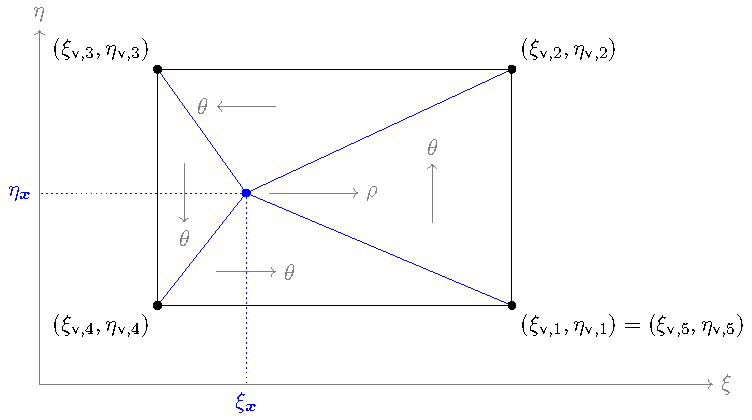
\includegraphics{Duffy}
	\caption{\textbf{Numerical evaluation of the boundary integral equations}: The element containing the source point $\vec{x}$ is divided in (up to) 4 triangles in the parameter domain.}
	\label{Fig3:Duffy}
\end{figure}
Each triangular sub element is divided into $n_{\mathrm{div},\uptheta}^{(i)}$ sub elements (in the $i^{\mathrm{th}}$ triangle) in the $\theta$-direction and $n_{\mathrm{div},\mathrm{r}}$ sub elements in the radial direction, where
\begin{equation*}
	n_{\mathrm{div},\uptheta}^{(i)} = \ceil{s_2\frac{\theta_{\mathrm{dir}}^{(i)}}{\ang{90}}},\quad n_{\mathrm{div},\mathrm{r}} = \ceil{s_2},\quad s_2 = \frac{\check{p}_{\mathrm{max}}+1+n_{\mathrm{eqp},2}}{2(\check{p}_{\mathrm{max}}+1)}.
\end{equation*}
Here, $\theta_{\mathrm{dir}}^{(i)}$ is the interior angle (in the parent domain) neighboring the source point of the initial sub triangle $i$. The reason for the subdivision of the triangles (as opposed to use high order quadrature) is that a high number of quadrature points is here needed (which will later be illustrated). This subdivision maps each sub element (in the $(\rho,\theta)$-domain) to the reference domain $[-1,1]^2$ by the linear transformation
\begin{equation}
\begin{aligned}
	\rho &= \rho_j + \frac12(\rho_{j+1}-\rho_j)(\tilde{\rho}+1),\qquad\rho_j = \frac{j}{n_{\mathrm{div},\mathrm{r}}},\qquad j=0,\dots,n_{\mathrm{div},\mathrm{r}}-1\\
	\theta &= \theta_l + \frac12(\theta_{l+1}-\theta_l)(\tilde{\theta}+1),\qquad\theta_l=\frac{l}{n_{\mathrm{div},\uptheta}^{(i)}},\qquad l=0,\dots,n_{\mathrm{div},\uptheta}^{(i)}-1
\end{aligned}
\end{equation}
with Jacobian determinant $J_3=1/(4n_{\mathrm{div},\uptheta}^{(i)}n_{\mathrm{div},\mathrm{r}})$. Each of these sub elements are now evaluated using $2(\check{p}_{\mathrm{max}}+1)$ quadrature points in both parametric directions.
%%%%%%%%%%%%%%%%%%%%%%%%%%%%%%%%%%%%%%%%%%

For the Galerkin formulations the integral integrating the BIEs uses $(\check{p}_\upxi+1+n_{\mathrm{eqp},1})\times(\check{p}_\upeta+1+n_{\mathrm{eqp},1})$ quadrature points over each element. If not otherwise stated, we shall use $n_{\mathrm{eqp},1}=0$ throughout this work.

In~\Cref{Fig3:Quadrature1,Fig3:Quadrature2} the locations of the quadrature points are illustrated on the third uniform mesh refinement of the coarse mesh in~\Cref{Fig3:sphere} (with $\check{p}=2$). 
\begin{figure}
	\begin{subfigure}[t]{\textwidth}
		\centering
		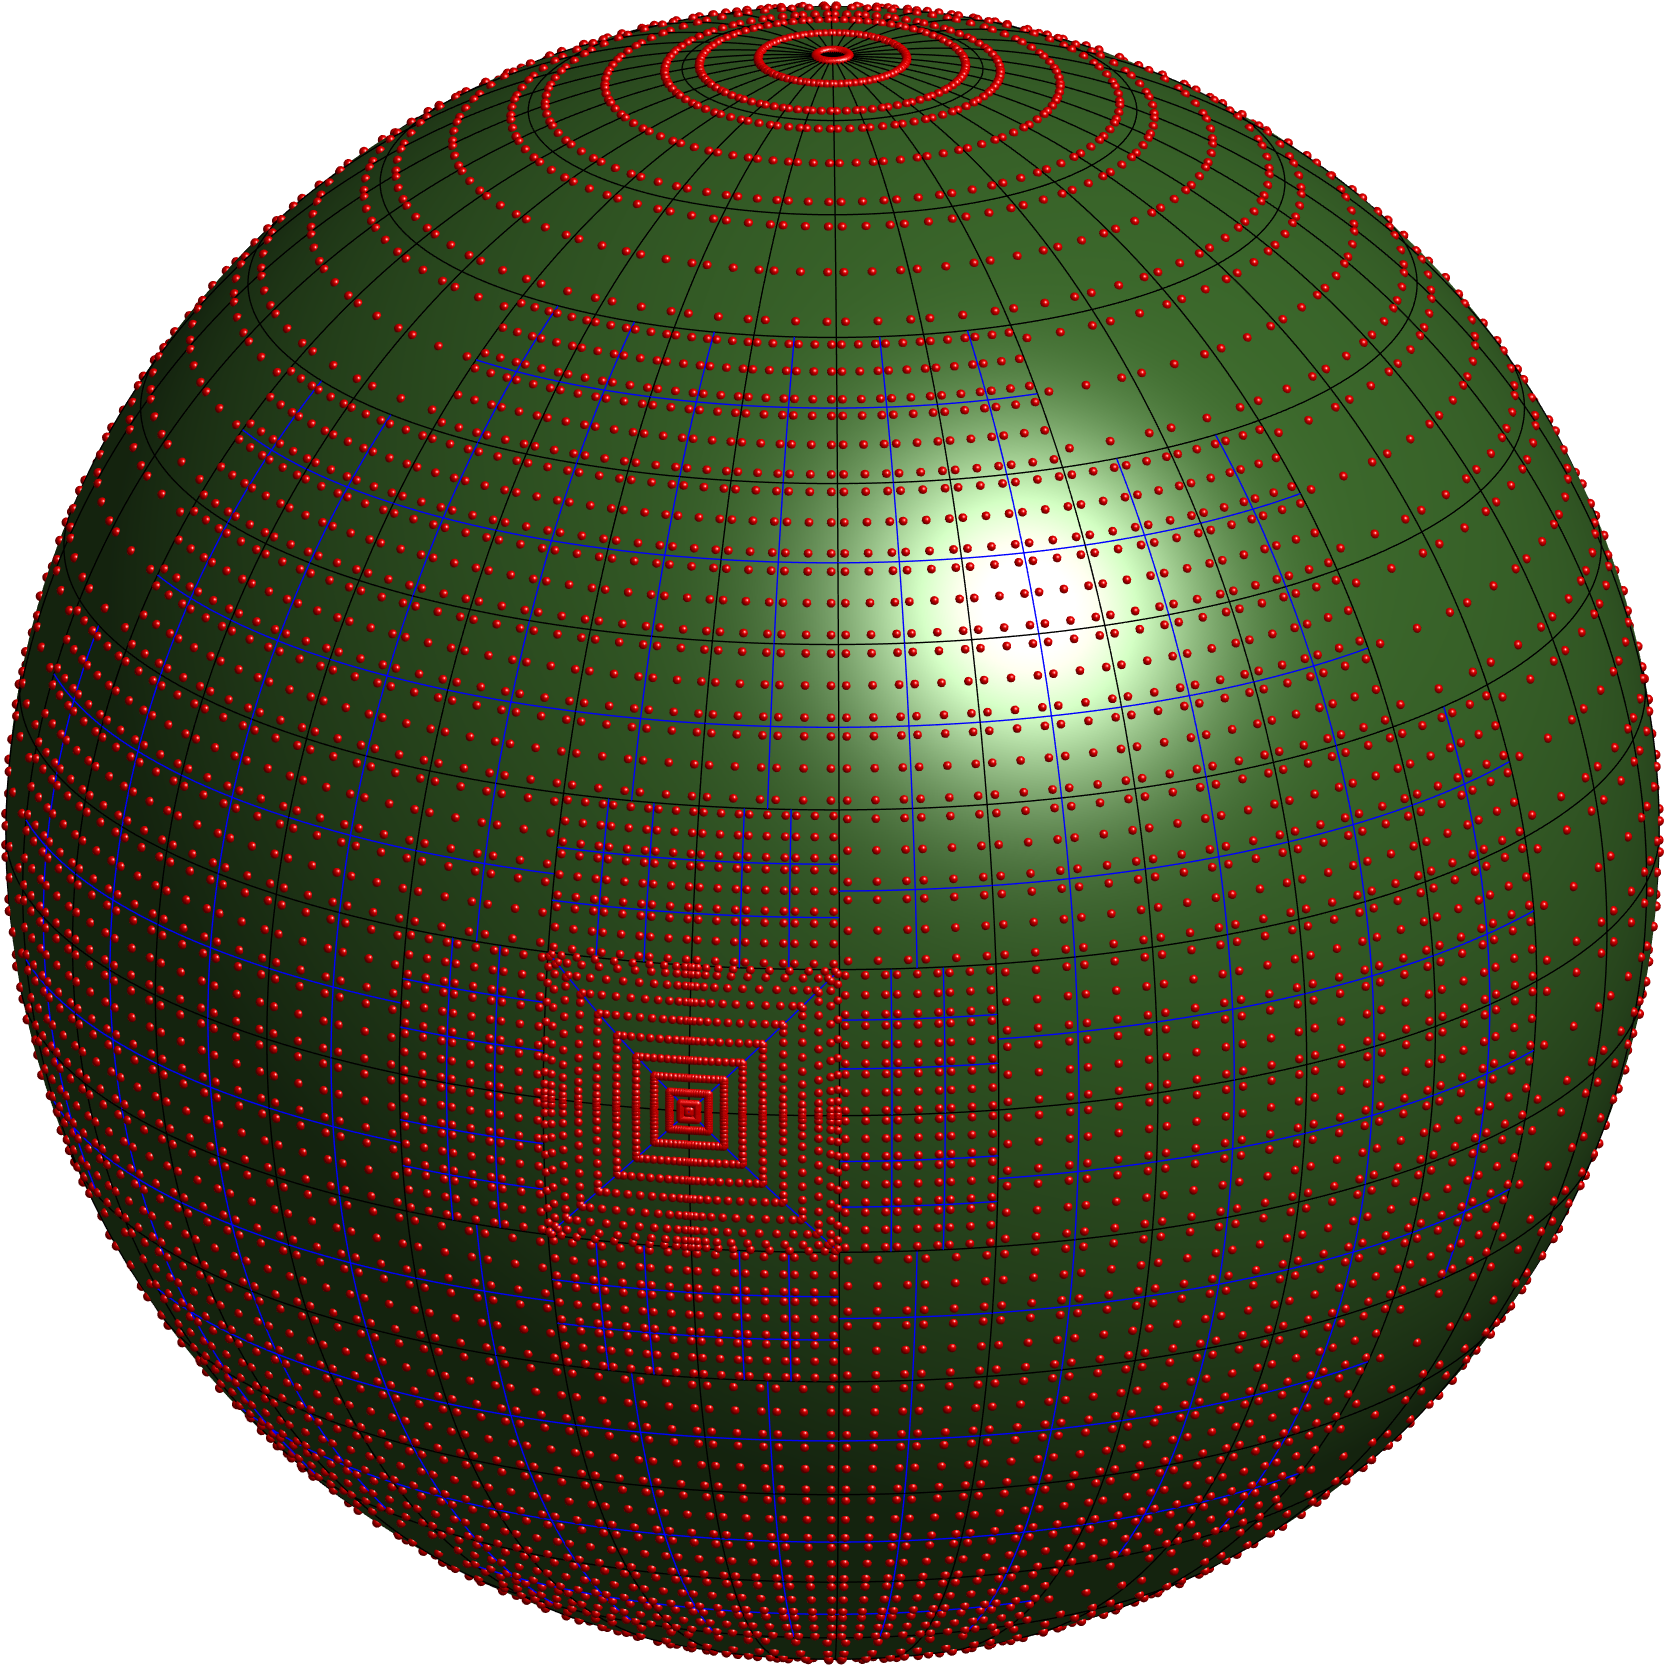
\includegraphics[width=0.49\textwidth]{S1_317_extraGPBEM8_agpBEM2_Simpson}%
		\hspace*{0.02\textwidth}%
		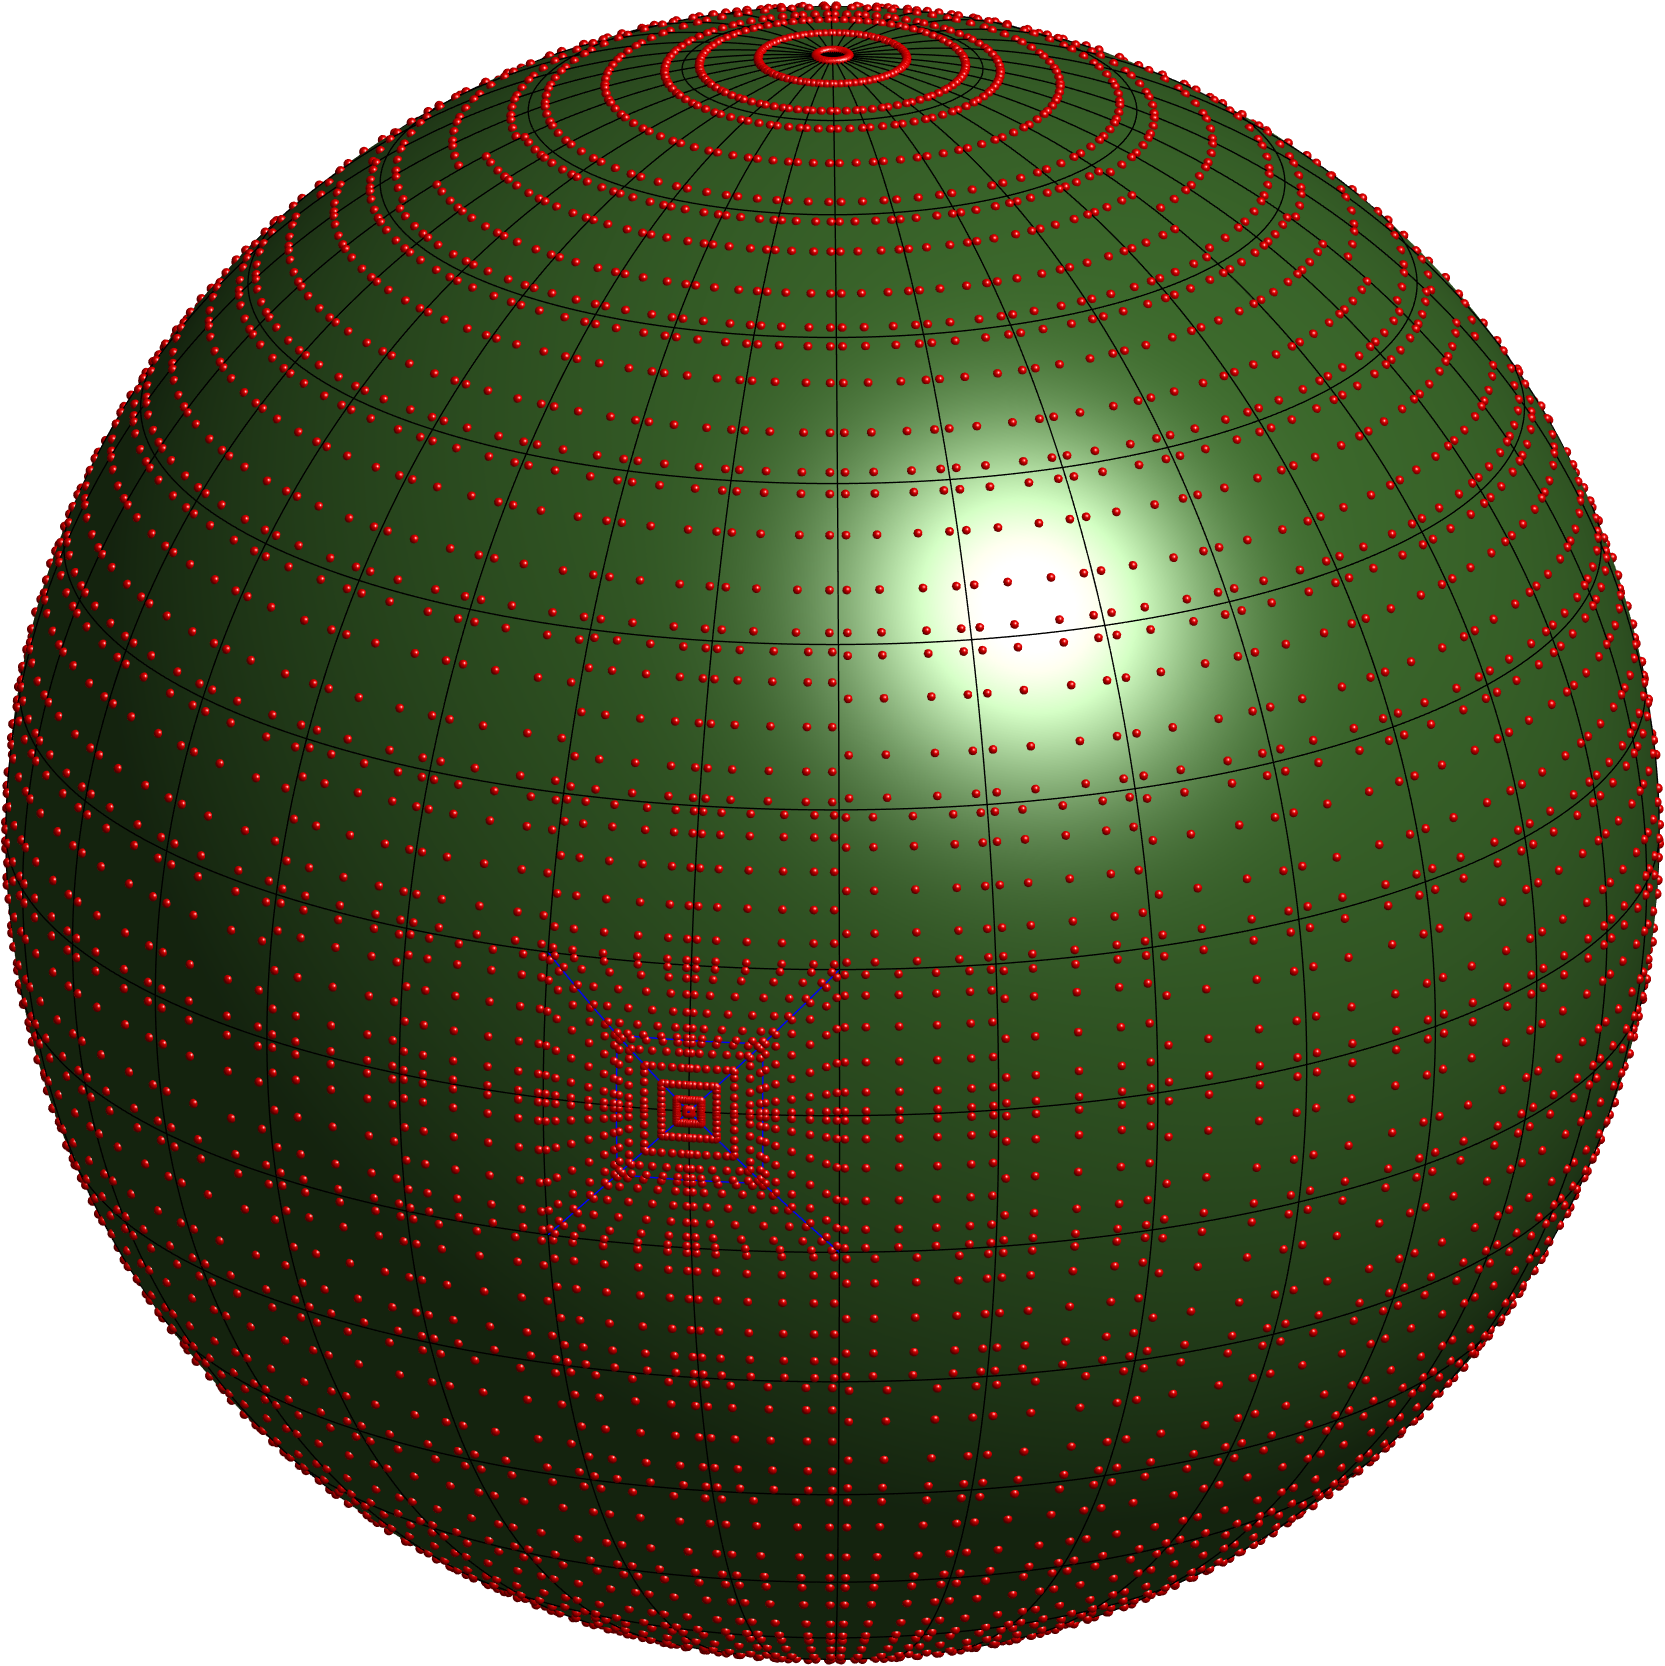
\includegraphics[width=0.49\textwidth]{S1_317_extraGPBEM8_agpBEM1_Adaptive2}
		\caption{The $317^{\mathrm{th}}$ collocation point is at a vertex shared by four elements.}
	\end{subfigure}
	\par\bigskip
	\par\bigskip
	\begin{subfigure}[t]{\textwidth}
		\centering
		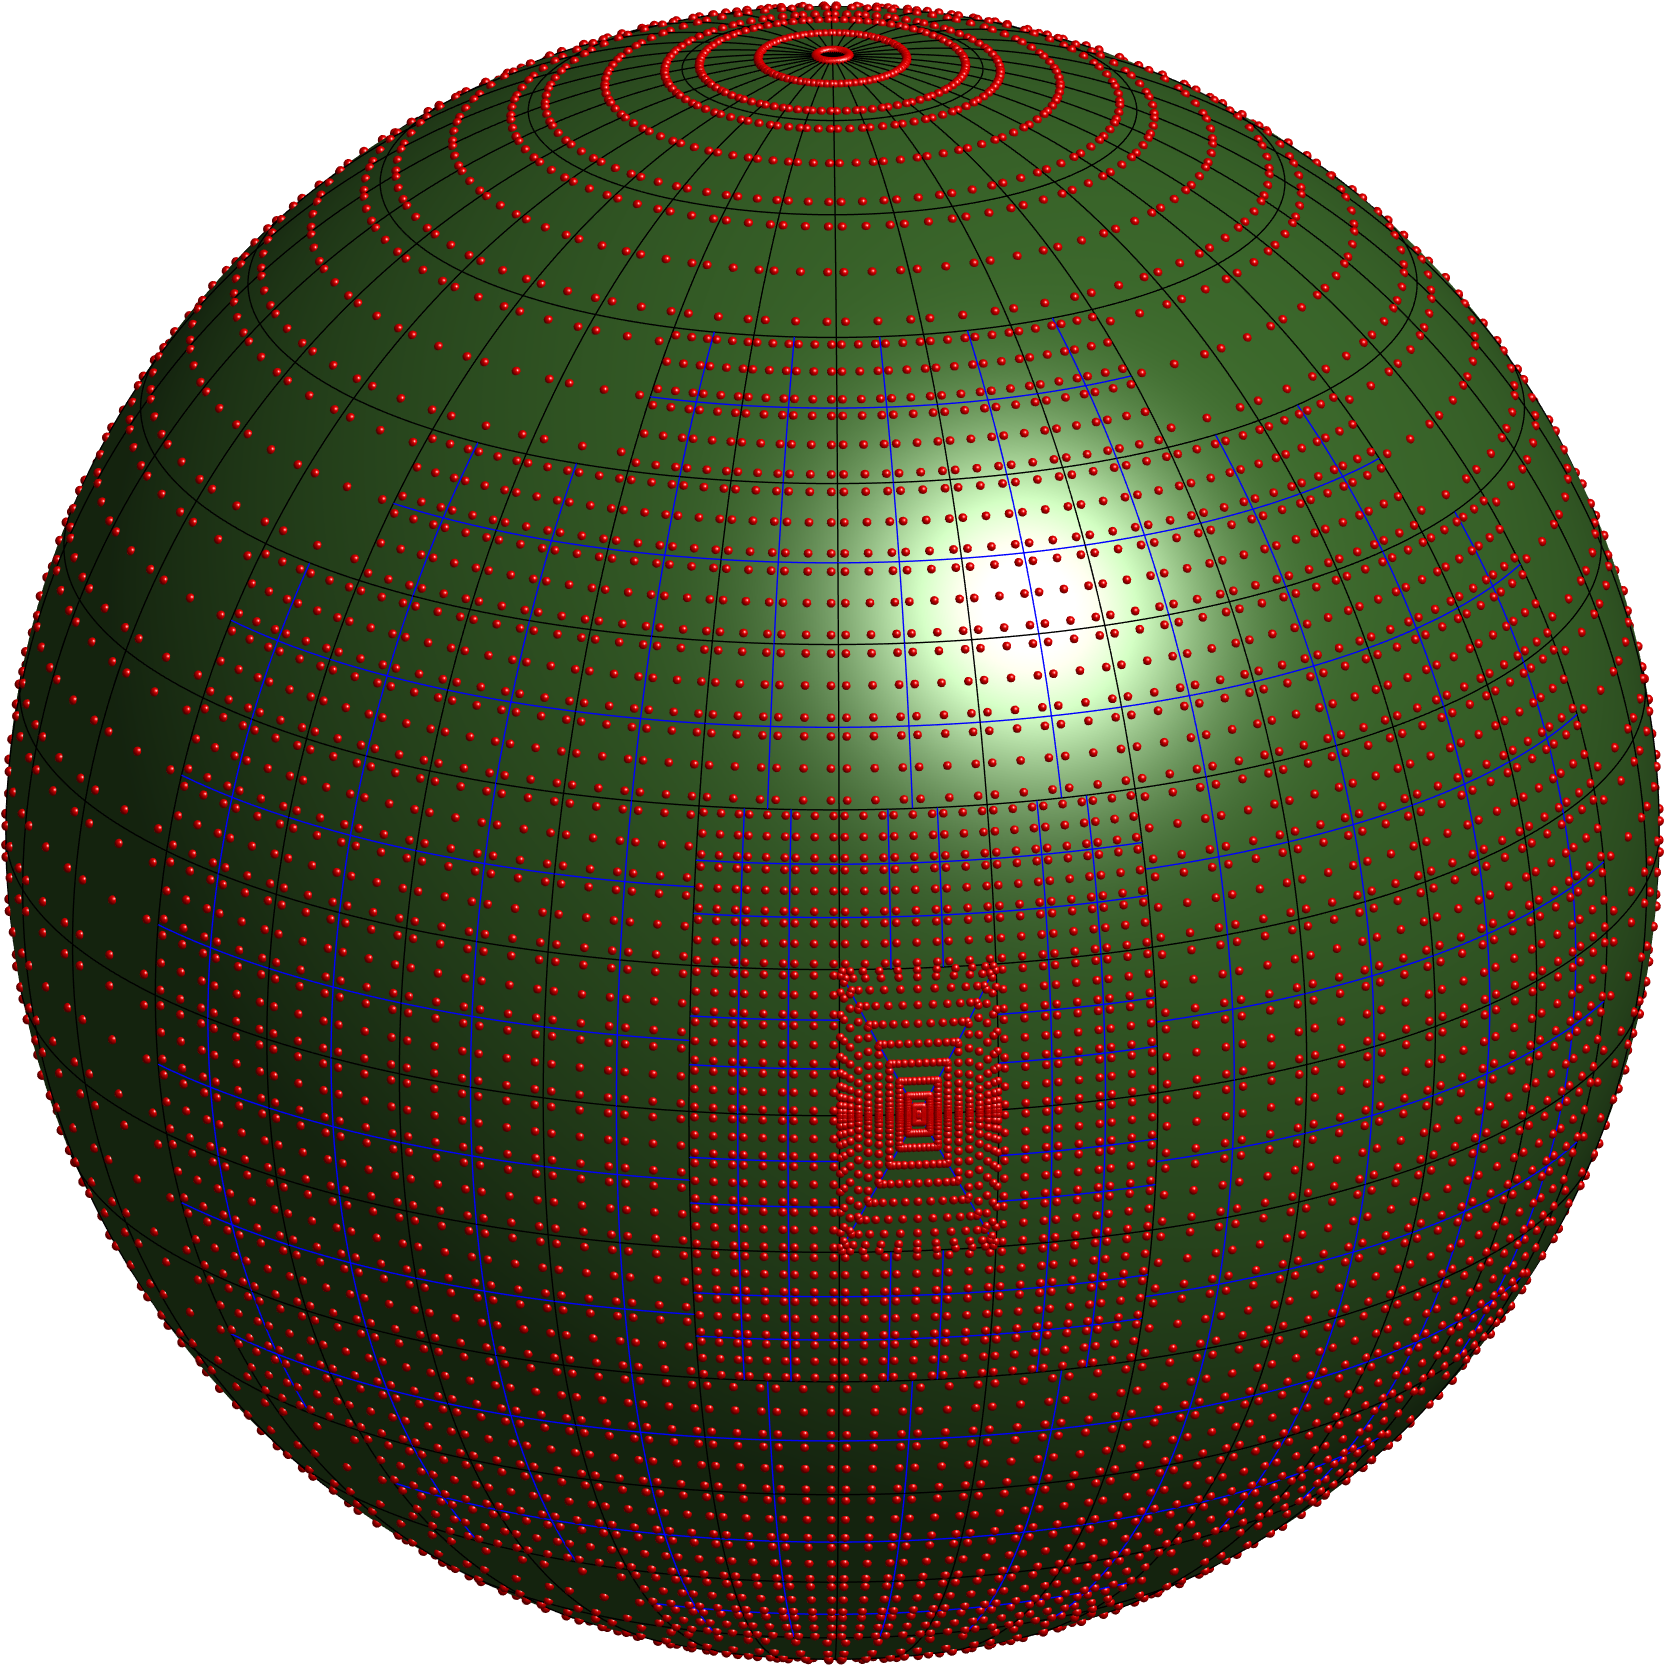
\includegraphics[width=0.49\textwidth]{S1_319_extraGPBEM8_agpBEM2_Simpson}%
		\hspace*{0.02\textwidth}%
		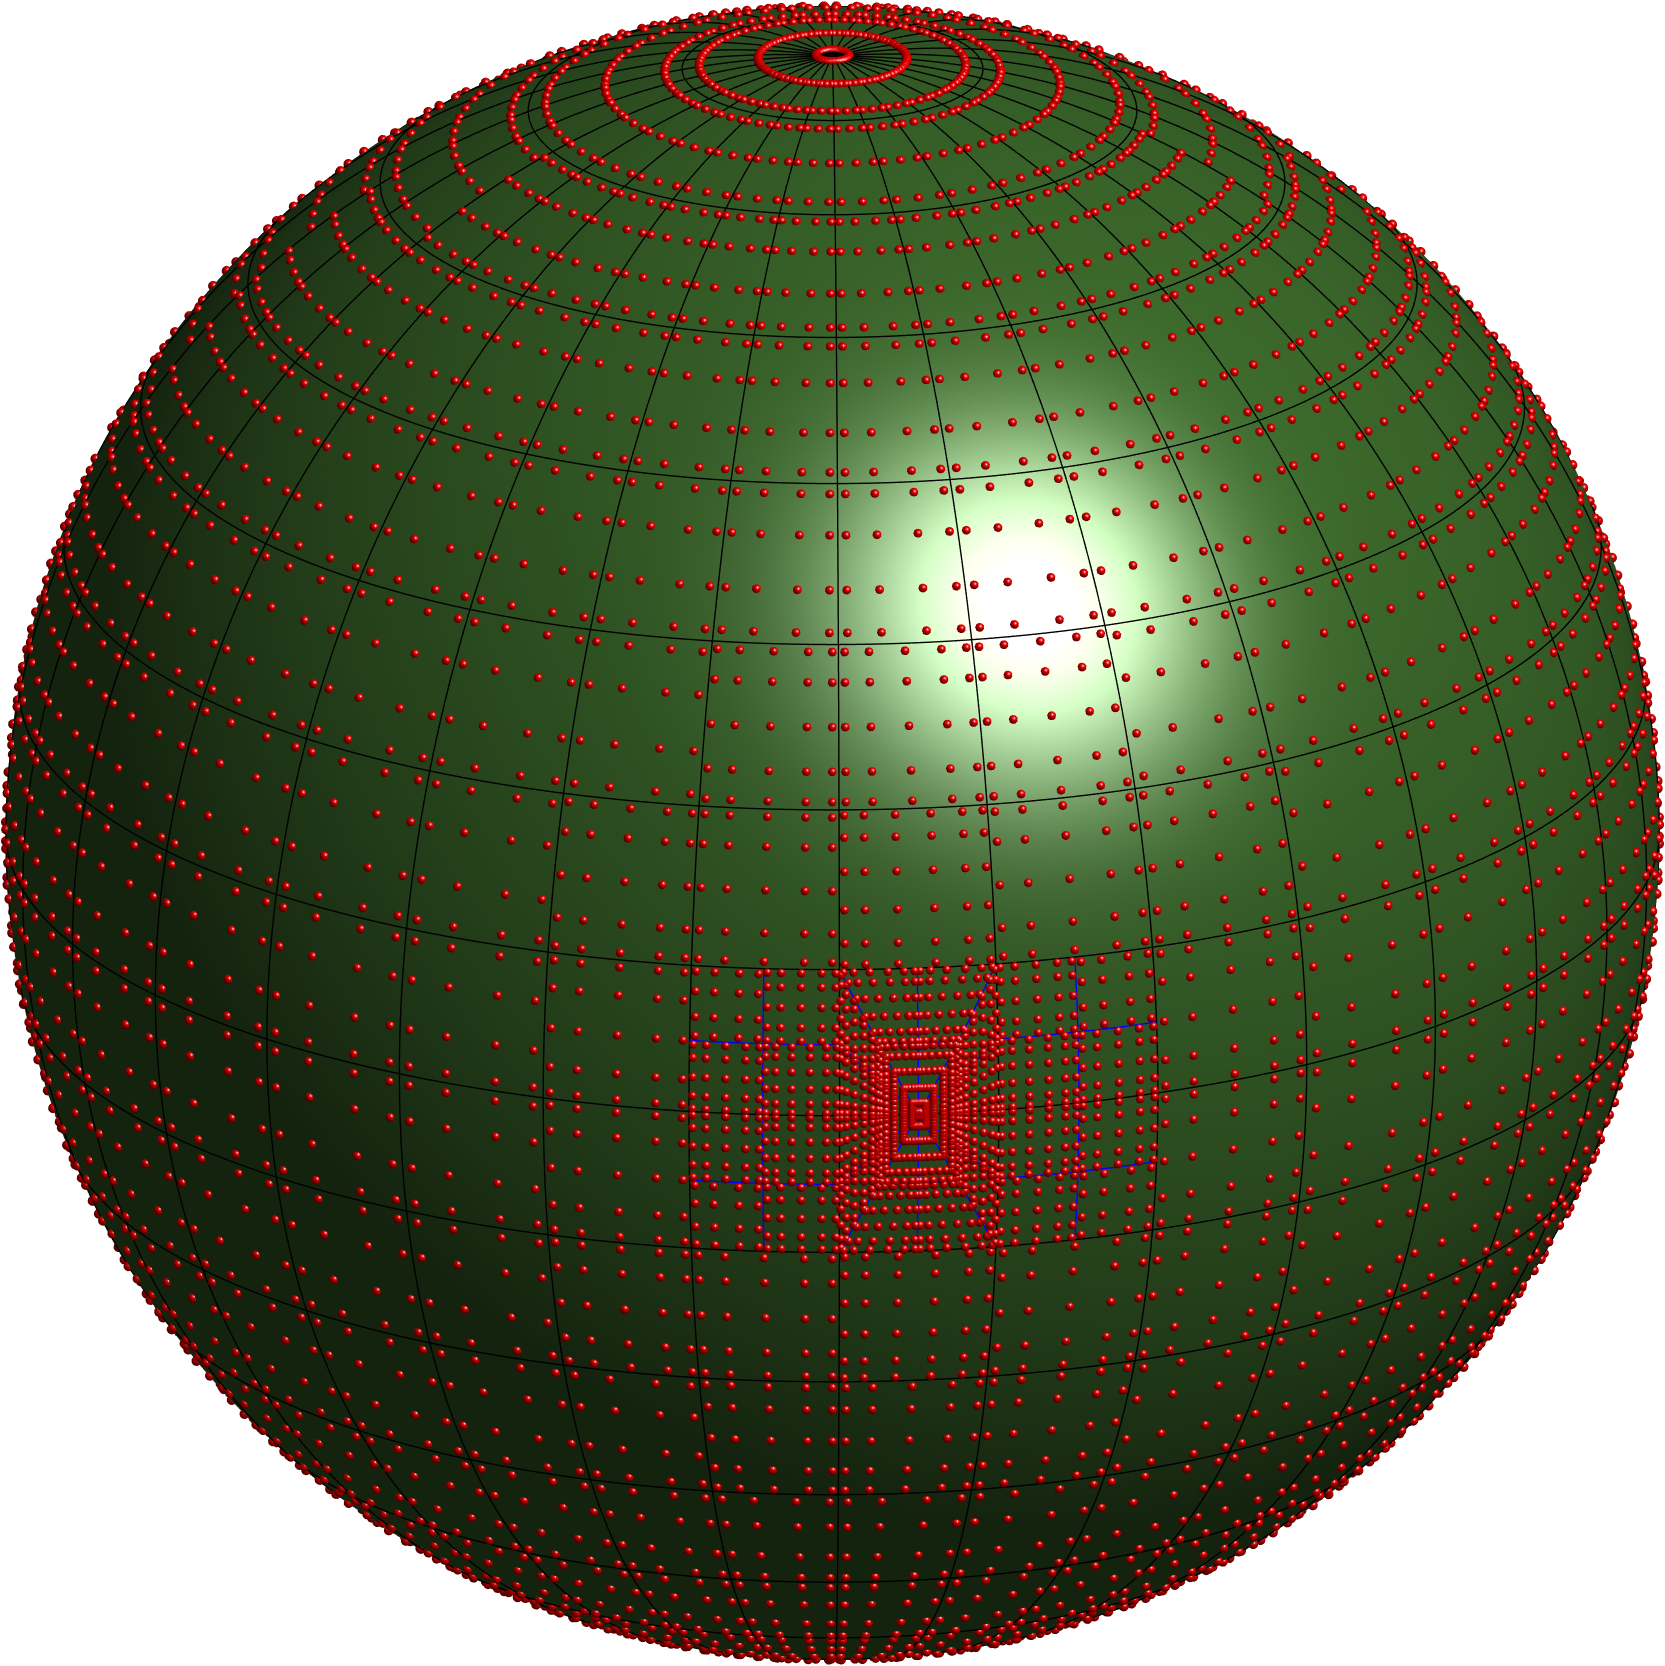
\includegraphics[width=0.49\textwidth]{S1_319_extraGPBEM8_agpBEM1_Adaptive2}
		\caption{The $319^{\mathrm{th}}$ collocation point is on an element edge shared by two elements.}
	\end{subfigure}
	\caption{\textbf{Numerical evaluation of the boundary integral equations}: The figures to the left are the integration procedure in~\cite{Simpson2014aib} (with $s_1=2$). The sub-element divisions are here shown by blue lines (the black lines are the element edges). The red points are the quadrature points. Here, $n_{\mathrm{eqp},1}=0$ and $n_{\mathrm{eqp},2}=8$, and we thus get $(\check{p}_{\mathrm{max}}+1+n_{\mathrm{eqp},2})\times(\check{p}_{\mathrm{max}}+1+n_{\mathrm{eqp},2})=11\times 11$ quadrature in each sub-element around the source point, and $(\check{p}_\upxi+1+n_{\mathrm{eqp},1})\times(\check{p}_\upeta+1+n_{\mathrm{eqp},1})=3\times 3$ in the remaining elements. The figures to the right are the new integration routine presented in this work with $s_1=1$.}
	\label{Fig3:Quadrature1}
\end{figure}
\begin{figure}
	\begin{subfigure}[t]{\textwidth}
		\centering
		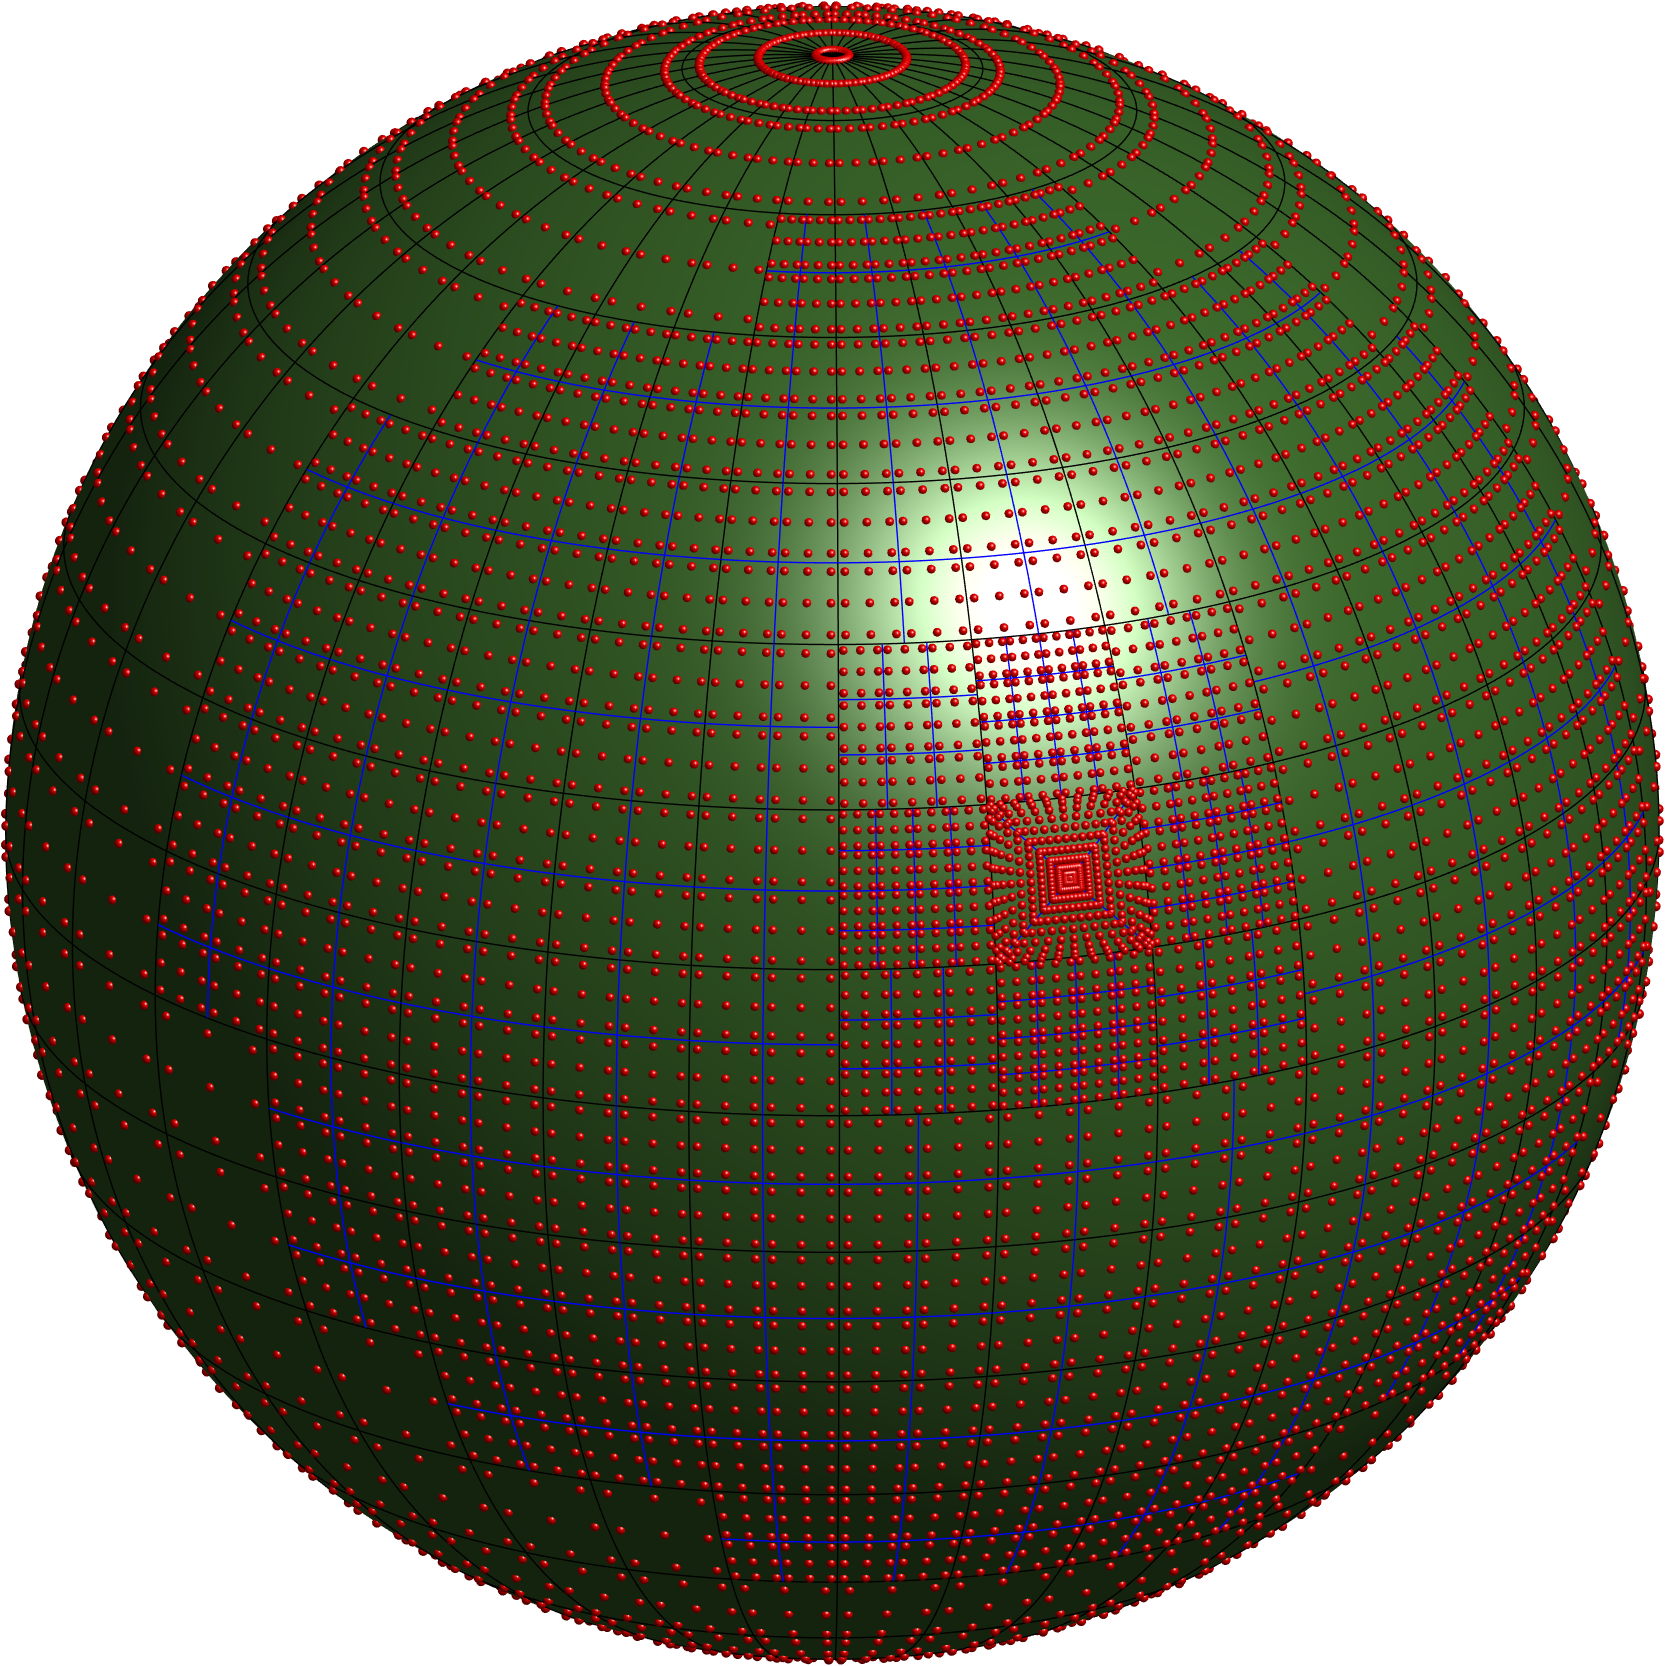
\includegraphics[width=0.49\textwidth]{S1_392_extraGPBEM8_agpBEM2_Simpson}%
		\hspace*{0.02\textwidth}%
		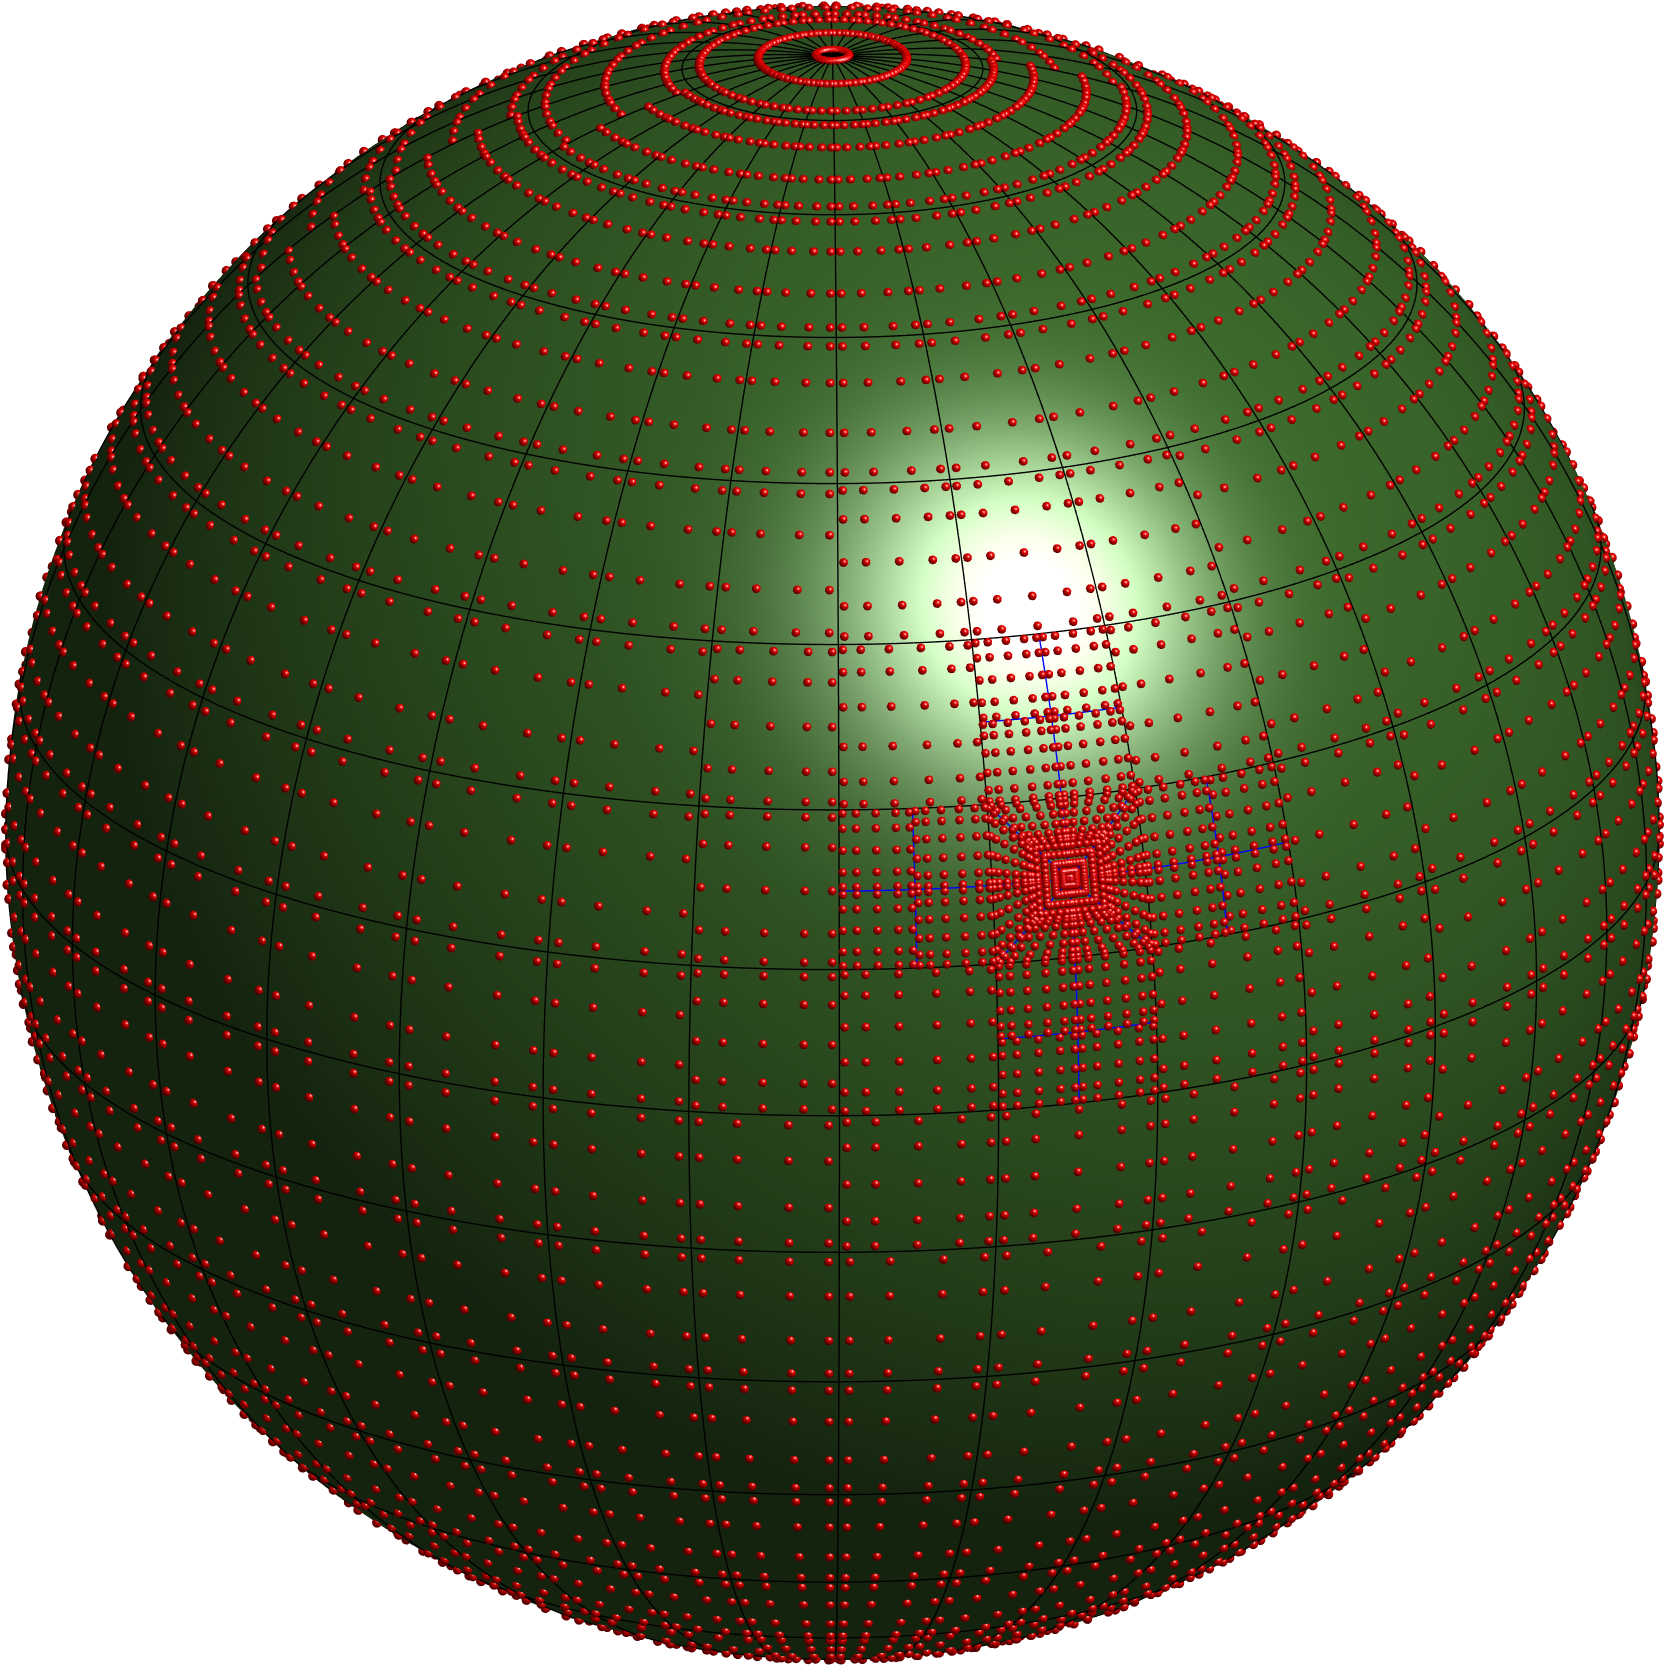
\includegraphics[width=0.49\textwidth]{S1_392_extraGPBEM8_agpBEM1_Adaptive2}
		\caption{The $392^{\mathrm{th}}$ collocation point is at the center of an element.}
	\end{subfigure}
	\par\bigskip
	\par\bigskip
	\begin{subfigure}[t]{\textwidth}
		\centering
		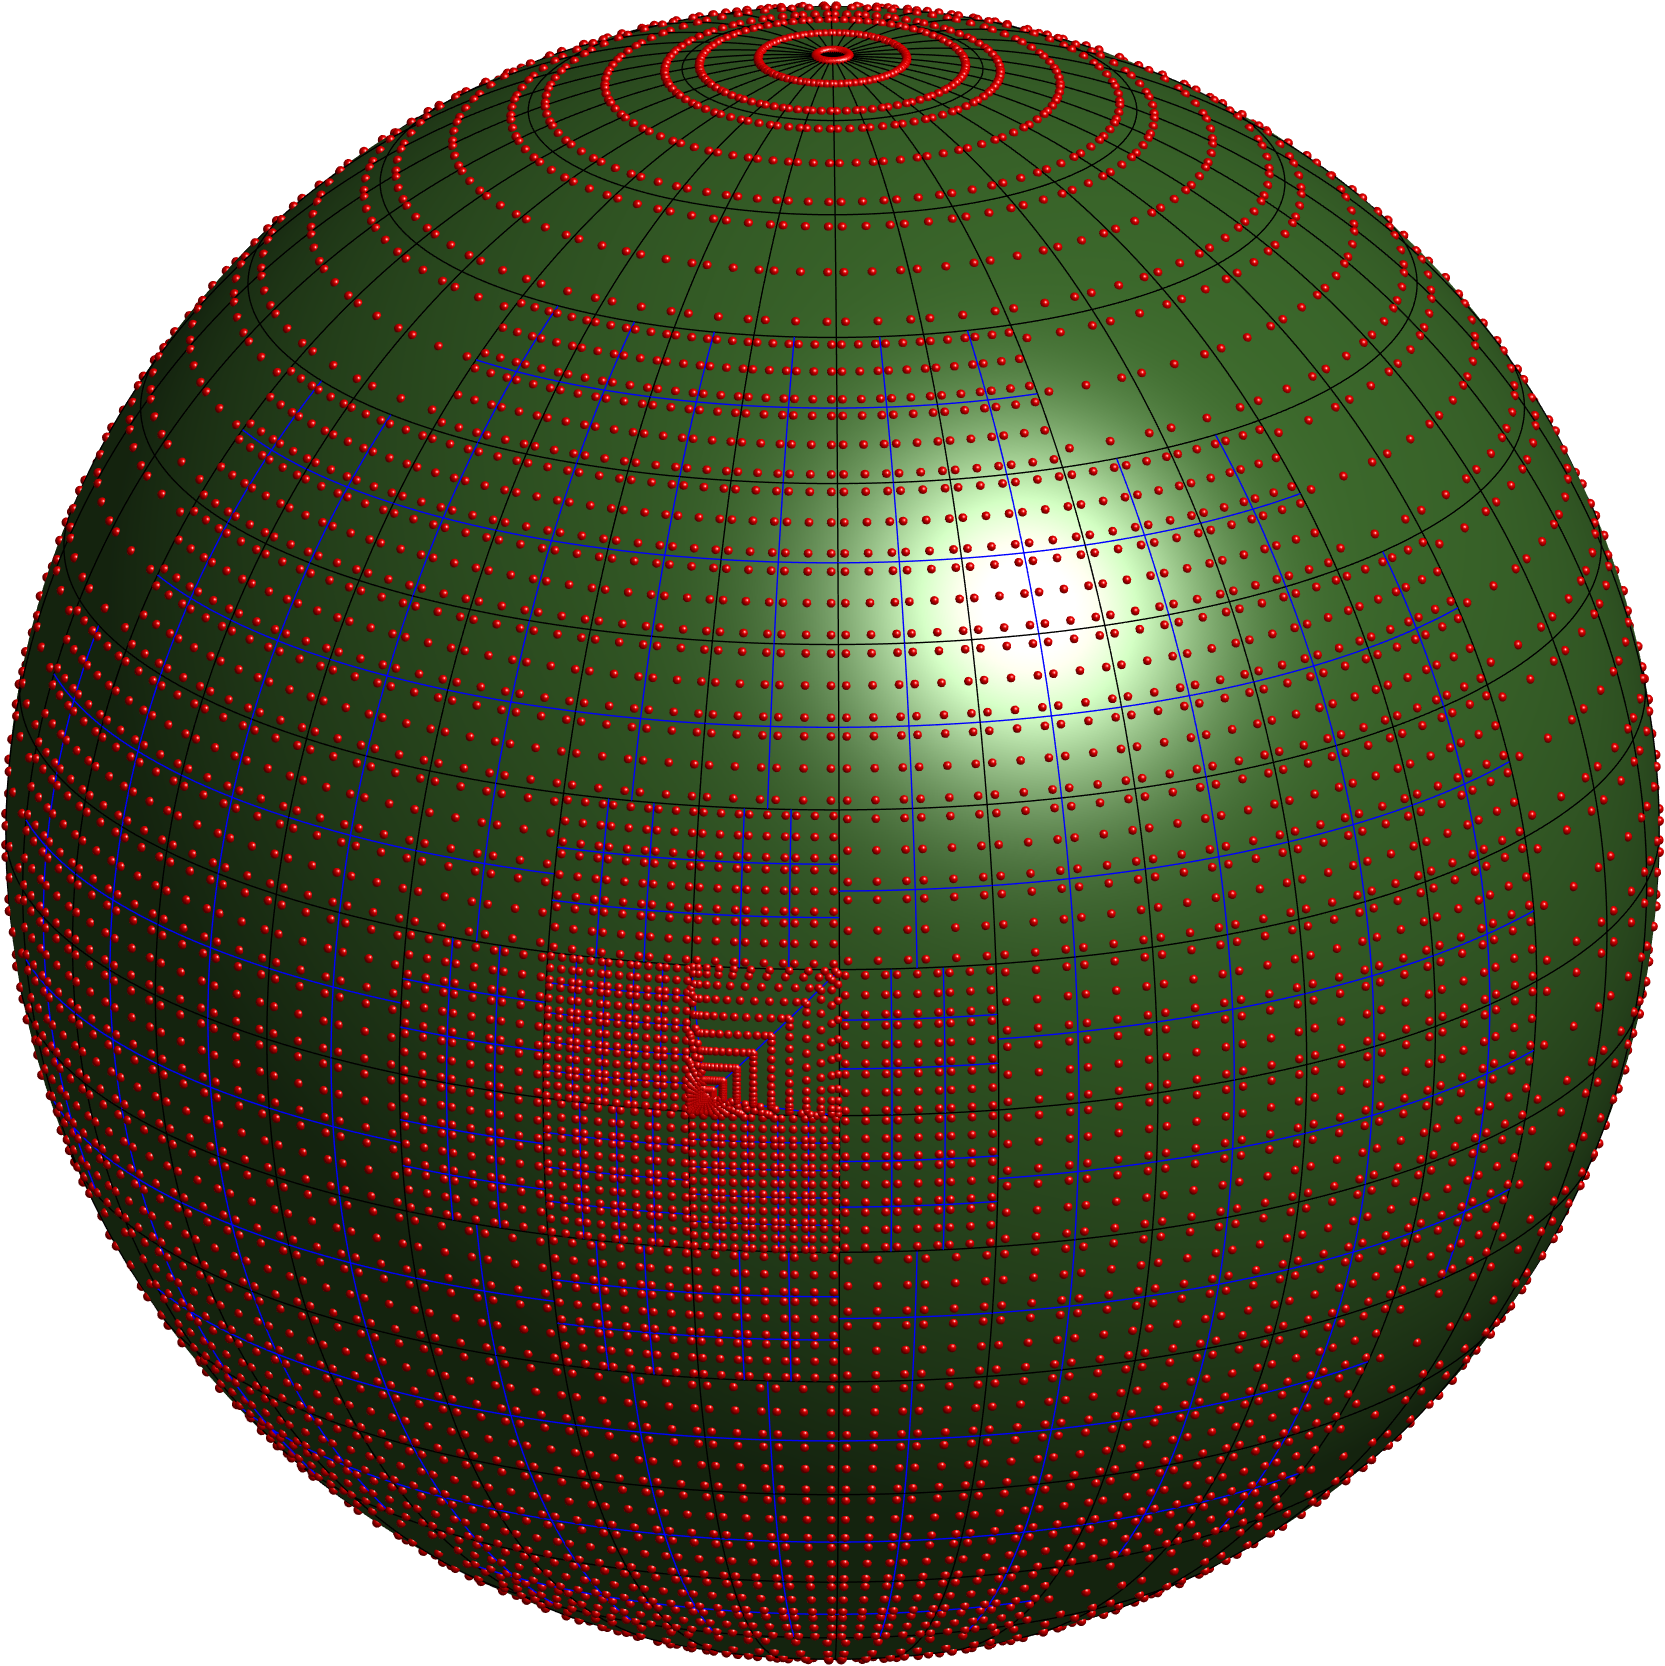
\includegraphics[width=0.49\textwidth]{S1_354_extraGPBEM8_agpBEM2_Simpson}%
		\hspace*{0.02\textwidth}%
		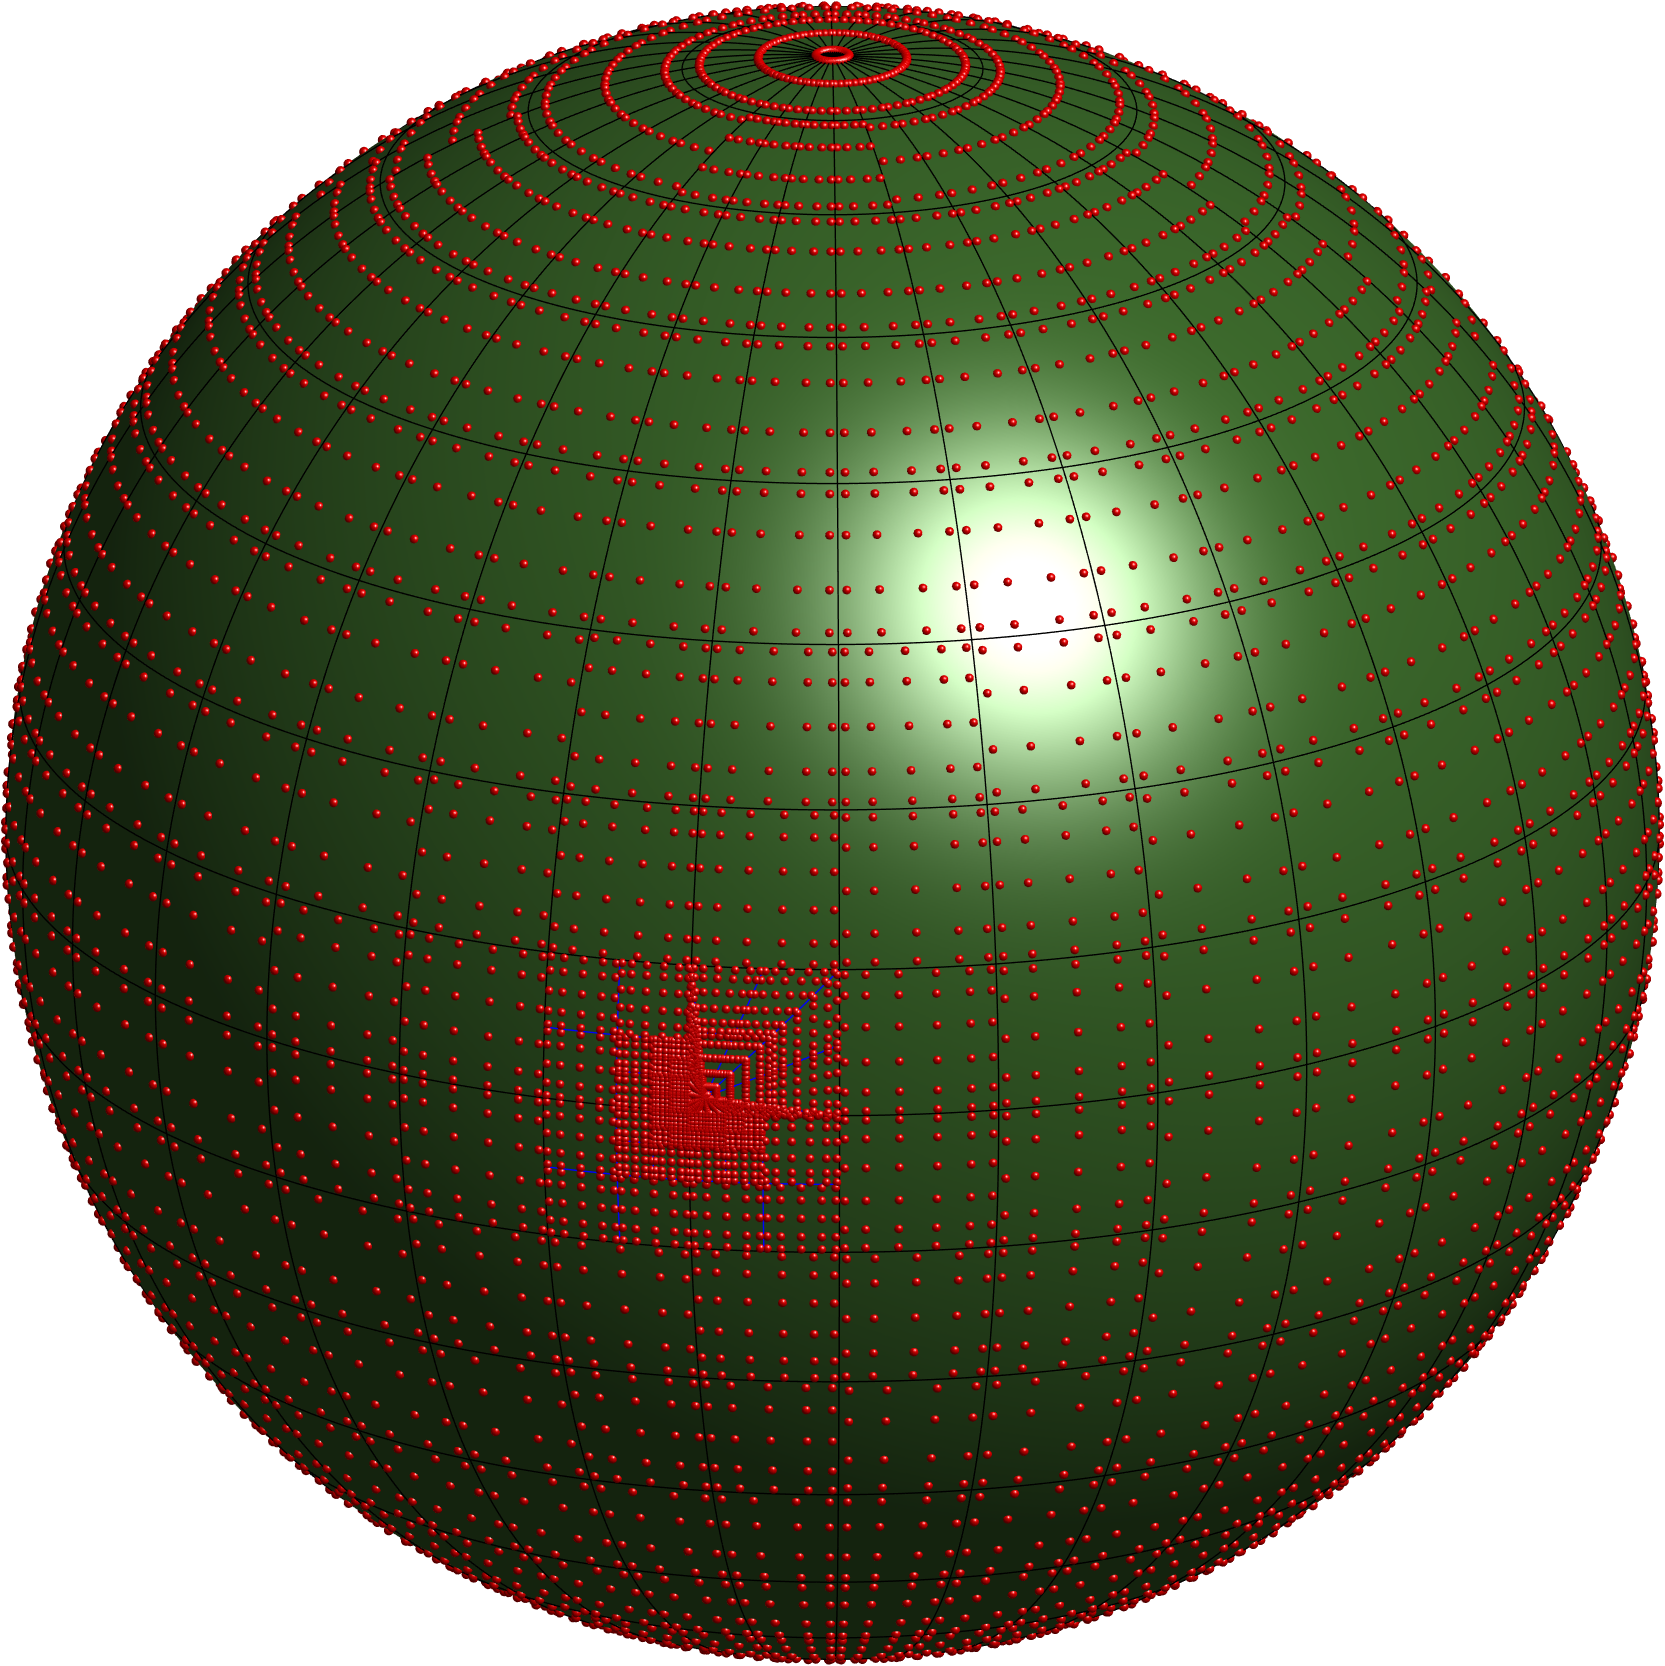
\includegraphics[width=0.49\textwidth]{S1_354_extraGPBEM8_agpBEM1_Adaptive2}
		\caption{The source point is the corner quadrature point for Galerkin formulations inside an element.}
	\end{subfigure}
	\caption{\textbf{Numerical evaluation of the boundary integral equations}: The figures to the left are the integration procedure in~\cite{Simpson2014aib} (with $s_1=2$). The sub-element divisions are here shown by blue lines (the black lines are the element edges). The red points are the quadrature points. Here, $n_{\mathrm{eqp},1}=0$ and $n_{\mathrm{eqp},2}=8$, and we thus get $(\check{p}_{\mathrm{max}}+1+n_{\mathrm{eqp},2})\times(\check{p}_{\mathrm{max}}+1+n_{\mathrm{eqp},2})=11\times 11$ quadrature in each sub-element around the source point, and $(\check{p}_\upxi+1+n_{\mathrm{eqp},1})\times(\check{p}_\upeta+1+n_{\mathrm{eqp},1})=3\times 3$ in the remaining elements. The figures to the right are the new integration routine presented in this work with $s_1=1$.}
	\label{Fig3:Quadrature2}
\end{figure}